 \documentclass[xcolor=dvipsnames]{beamer}
\usepackage{amsmath,amssymb,amsfonts,latexsym,stmaryrd}
\usepackage{listings}
\usepackage{epstopdf}
\usepackage[latin1]{inputenc}
\usepackage{multimedia}
\usepackage[T1]{fontenc}
\usetheme{metropolis}
%\usetheme{Pittsburgh}
%\usetheme[purple]{bearmetheme-light}
%\usetheme[numbering=none]{focus}
\usepackage{times}
\usepackage{tikz}
\usepackage{verbatim}
\usetikzlibrary{arrows,shapes}
\usepackage{multicol}
\usepackage{braket}

% #####            #####
%     DATOS DE TITULO
% #####            #####

\author{Shigueru Nagata }
\date{2019}
\title{C\'alculos de estructura electr\'onica en perovskitas $BiFeO_{3}$ y 
$YCrO_{3}$}
\institute{Universidad Nacional de Ingenier\'ia \\ Facultad de ciencias}

\begin{document}
    
% ----- TITULO ----
    \begin{frame}
        \titlepage
    \end{frame}

% ----- Indice ----

\begin{frame}
    \frametitle{\'Indice}
    \begin{multicols}{2}
        \begin{enumerate}
            \item Introducci\'on
            \item Conceptos b\'asicos
                \begin{itemize}
                    \item Aproximaci\'on de Born-Oppenheimer
                    \item M\'etodo de Hartree-Fock
                    \item Teoremas de Hohenberg-Kohn
                    \item Ecuaci\'on de Kohn-Sham
                    \item Aproximaci\'on de densidad local
                    \item Par\'ametro U de Hubbard
                    \item Pseudopotencial
                    \item Arreglos antiferromagn\'eticos
                    \item Bucle autoconsistente
                \end{itemize}
            \item Resultados
                \begin{itemize}
                    \item Optimizaci\'on de par\'ametros iniciales
                    \item Relajaci\'on de la estructura cristalina
                    \item Bandas de energ\'ia y densidades de estado
                    \item Comparaci\'on entre $BiFeO_{3}$ y $YCrO_{3}$
                \end{itemize}
            \item Conclusiones
        \end{enumerate}
    \end{multicols}
\end{frame}

\section{Introducci\'on}
\begin{frame}{}
    \begin{columns}[t]
        \column{0.33\textwidth}
\textbf{Multiferroicos}
\begin{itemize}
    \item {\small Ferroelectricidad}
    \item {\small Ferromagnetismo}
    \item {\small Ferroelasticidad}
    \end{itemize}
        \column{0.33\textwidth}
\textbf{Aplicaciones}
\begin{itemize}
    \item {\small Sensores}
    \item {\small Transductores}
    \item {\small Osciladores}
    \item {\small Dispositivo de almacenamiento}
\end{itemize}
        \column{0.33\textwidth}
{\small El $BiFeO_{3}$ y $YCrO_{3}$ han sido sintetizados en el Laboratorio de F\'isica de la Materia Condensada (LFMC) de la Universidad Nacional de Ingenier\'ia.}
    \end{columns}
\end{frame}

% #####            #####
%        TEORIA
% #####            ##### 

\section{Conceptos b\'asicos}

% ======================
% Aproximacion Born-Openheimer
% ======================

\subsection{Aproximaci\'on de Born-Oppenheimer}
\begin{frame}{Hamiltoniano}
    \begin{eqnarray}
    -\sum _{I=1}^{N} \frac{1}{2} \nabla _{I}^{2} - \sum 
    _{i=1}^{n} \frac{1}{2} \nabla _{i}^{2} + \frac{1}{2} \sum _{I \ne 
        J}^{N} \frac{Z_{I}Z_{J}}{|R_{I}-R_{J}|} + \frac{1}{2} \sum _{i\ne 
        j}^{n} \frac{1}{|r_{i}-r_{j}|} - \nonumber \\ 
     \sum _{I}^{N} \sum _{j}^{n} \frac{Z_{I}}{|R_{I}-r_{j}|} \nonumber
    \end{eqnarray}
    
\begin{itemize}
    \item $-\sum _{I=1}^{N} \frac{1}{2} \nabla _{I}^{2}$ : 
    Energ\'ia cin\'etica de los n\'ucleos.
    \item $- \sum _{i=1}^{n} \frac{1}{2} \nabla _{i}^{2}$ : 
    Energ\'ia cin\'etica de los electrones.
    \item $\frac{1}{2} \sum _{I \ne J}^{N} 
    \frac{Z_{I}Z_{J}}{|R_{I}-R_{J}|}$ : 
    Interacci\'on n\'ucleo-n\'ucleo.
    \item $\frac{1}{2} \sum _{i\ne j}^{n} 
    \frac{1}{|r_{i}-r_{j}|}$ : 
    Interacci\'on electr\'on-electr\'on.
    \item $\sum _{I}^{N} \sum _{j}^{n} 
    \frac{Z_{I}}{|R_{I}-r_{j}|}$ : 
    Interacci\'on n\'ucleo-electr\'on.
\end{itemize}

\end{frame}

\begin{frame}{Aproximaci\'on Born-Oppenheimer}
    \begin{eqnarray}
    H_{BO} =-\sum _{i=1}^{N} \frac{1}{2} \nabla _{i}^{2} + \frac{1}{2} \sum _{I 
    \ne 
        J}^{N} \frac{Z_{I}Z_{J}}{|R_{I}-R_{J}|} + \frac{1}{2} \sum _{i\ne 
        j}^{n} 
    \frac{1}{|r_{i}-r_{j}|} - \nonumber \\ \sum _{I}^{N} \sum _{j}^{n} 
    \frac{Z_{I}}{|R_{I}-r_{j}|} \nonumber
    \end{eqnarray}
\begin{itemize}
    \item Nucleos fijos
    \item Los nucleos dan origen al potencial externo donde se mueven los 
    electrones.
\end{itemize}
\end{frame}

% ======================
% Hartree-Fock
% ======================

\subsection{M\'etodo de Hartree-Fock}
\begin{frame}{M\'etodo de Hartree-Fock}
    
    \begin{block}{Determinante de Slater}
        \begin{equation}
        \psi (r_{1}r_{2}\cdots r_{N}) = \frac{1}{\sqrt{N!}} 
        \left ( 
        \begin{array}{cccc}
        \phi _{1}(r_{1}) & \phi _{2}(r_{1}) & \cdots & \phi _{N}(r_{1}) \\
        \phi _{1}(r_{2}) & \phi _{2}(r_{2}) & \cdots & \phi _{N}(r_{2}) \\
        \vdots & \vdots & \ddots & \vdots \\
        \phi _{1}(r_{N}) & \phi _{2}(r_{N}) & \cdots & \phi _{N}(r_{N})
        \end{array} 
        \right ) \nonumber
        \end{equation}
    \end{block}
    
    \begin{block}{Ecuaci\'on de Hartree-Fock}
        \begin{eqnarray}
        \big [ - \sum _{i}^{n} \frac{1}{2} \nabla _{i}^{2} - \sum _{i} ^{N} 
        \frac{Z_{i}}{|R_{i}-r|} + \sum _{i \ne j} ^{n} \int \frac{|\phi 
            _{i}(r^{\prime})|^{2}}{|r-r^{\prime }|}d^{3}r^{\prime} \big] \phi 
            _{j} 
        (r) \nonumber \\ - \sum _{i} \int dr^{\prime} \frac{\phi 
            _{i}^{*}(r^{\prime}) \phi 
            _{j}(r^{\prime})}{|r^{\prime}-r|} \phi_{i}(r) = E_{j} \phi _{j}(r) 
        \nonumber
        \end{eqnarray}
    \end{block}
    
\end{frame}

% ======================
% Teoremas Hohenberg-Kohn
% ======================

\subsection{Teoremas de Hohenberg-Kohn}
\begin{frame}{Teoremas de Hohenberg-Kohn}
    \begin{block}{Teorema I}
        El potencial $V_{ext}(r)$ est\'a determinado \'unicamente, excepto por 
        una constante, por la densidad del estado fundamental $\rho _{0}(r)$.
    \end{block}

    \begin{block}{Teorema II}
    La densidad que minimiza la energ\'ia total es exactamente la densidad del 
    estado fundamental.
    \end{block}
\end{frame}

% ======================
% Ecuacion kohn-Sham
% ======================

\subsection{Ecuaci\'on de Kohn-Sham}
\begin{frame}{Ecuaci\'on de Kohn-Sham}
    \begin{equation}
    \left[ -\frac{1}{2}\nabla_{i}^{2} + V_{ext}  + V_{H} + V_{xc} \right] 
    \phi_{i}(r) = \varepsilon_{i} \phi_{i}(r) \nonumber
    \end{equation}
    \begin{itemize}
        \item $-\frac{1}{2}\nabla_{i}^{2}$ : Energ\'ia cinetica.
        \item $V_{ext}$ : Potencial externo.
        \item $V_{H}$ : Potencial de Hartree.
        \item $V_{xc}$ : Potencial de intercambio-correlaci\'on
    \end{itemize}
\end{frame}

% ======================
% Aproximacion densidad local
% ======================

\subsection{Aproximaci\'on de densidad local}
\begin{frame}{Aproximaci\'on de densidad local}
Permite aproximar el t\'ermino de intercambio-correlaci\'on.
\begin{eqnarray}
E_{xc}^{LDA} [\rho ] = \int d^{3}r \rho (r) \varepsilon _{xc}^{unif} [\rho 
(r)] \nonumber
\end{eqnarray}
\begin{columns}[t]
    \column{0.5\textwidth}
        \[   \varepsilon _{x}^{unif} (\rho ) = -\frac{3}{4} \left( \frac{3}{\pi 
        } \right) 
        ^{1/3} \rho ^{1/3}\]
    \column{0.5\textwidth}
    \\
    {\scriptsize Many-Particle Physics. Gerald D. Mahan pp.299}
\end{columns}

\begin{columns}[t]
    \column{0.7\textwidth}
\[    \varepsilon _{c}^{unif} (\rho ) = \left\{ \begin{array}{ll}
A \ln r_{s} + B + C r_{s} \ln r_{s} & \textrm{; } r_{s} \to 0 \\ 
\frac{D}{r_{s}} + \frac{E}{r_{s}^{3/2}} & \textrm{; } r_{s} \to \infty
\end{array} \right.\]
\[
r_{s} = \left( \frac{3}{4\pi \rho} \right)^{1/3}
\]
    \column{0.3\textwidth}
    \\
$r_{s}$ : radio de wigner-Seitz \\
{\scriptsize S. H. Vosko et al, Can. J. Phys. 58, 1200 (1980)}
\end{columns}
\end{frame}


\subsection{Potencial U de Hubbard}
\begin{frame}{Par\'ametro U de Hubbard}
    Los orbitales \textbf{d} fuertemente correlacionados requieren una correcci\'on de la energ\'ia.
    \[
    E^{LDA+U} [\rho (r)]= E^{LDA} [\rho (r)] + 
    E^{Hubbard}[n_{mm^{\prime}}^{I\sigma}] - E^{dc}[n^{I\sigma}]
    \]
    Donde:
    
    \begin{itemize}
        \item $E^{LDA} [\rho (r)]$ funcional de la energ\'ia en LDA.
        \item $E^{Hubbard}[n_{mm^{\prime}}^{I\sigma}]$ correlaci\'on de los estados ocupados de los orbitales.
        \item $E^{dc}[n^{I\sigma}]$ energ\'ia de correlaci\'on, para evitar el doble conteo.
    \end{itemize}
\[
E^{LDA+U} [\rho (r)]= E^{LDA} [\rho (r)] + \sum _{I} \left[ \frac{U}{2} \sum 
_{m,\sigma \neq m^{\prime},\sigma ^{\prime}} n_{m}^{I\sigma} 
n_{m^{\prime}}^{I\sigma ^{\prime}} - \frac{U}{2} n^{I}(n^{I}-1) \right]
\]
\end{frame}

\begin{frame}
    {\bf C\'alculo de U: semi-emp\'irico}
    Se prueban varios valores de {\bf U} buscando que los resultados coincidan con datos experimentales.
    \begin{figure}[H]
        \centering
        \includegraphics[width=0.6\textwidth]{contenido/teoria/img_teoria/hubbars.png}
        \caption{Estructura de bandas con diferentes valores de U. Sheng Ju et al. J. Chem. Phys. 130, 214708 (2009)}
    \end{figure}
\end{frame}

\begin{frame}
    {\bf C\'alculo de U: respuesta lineal}
    \begin{columns}[t]
        \column{0.5\textwidth}
        Se aplica una perturbaci\'on $\alpha$ en la energ\'ia de los estados {\bf d}.
        \[ U = \chi _{0}^{-1} - \chi ^{-1} \]
        donde: \[ \chi  = \frac{d n}{d \alpha } \]
        $\alpha$ es peque\~no y en un intervalo alrededor de cero.

        {\scriptsize Cococcioni and Gironcoli (2005)}        \column{0.5\textwidth}
        Procedimiento en Quantum ESPRESSO:
        \begin{itemize}
            \item C\'alculo scf sin perturbaci\'on.
            \item C\'alculo scf con cada valor de $\alpha$.
        \end{itemize}
    \begin{figure}[H]
        \centering
        \includegraphics[width=1.0\textwidth]{contenido/teoria/img_teoria/RespuestaLineal.png}
    \end{figure}
\[ U = \chi _{0}^{-1} - \chi ^{-1} = 1/a_{0} - 1/a  \]
    \end{columns}
\end{frame}

% ======================
% Pseudopotencial
% ======================

\subsection{Pseudopotencial}
\begin{frame}{Pseudopotencial}
     \begin{columns}[t]
        \column{0.5\textwidth}
        \begin{figure}[H]
            \centering
            \includegraphics[width=1.0\textwidth]{contenido/teoria/img_teoria/pseudopotential.png}
            \caption{Representaci\'on del pseudopotencial}
        \end{figure}
        \column{0.5\textwidth}
        \begin{itemize}
            \item Reemplazo de las funciones de onda por pseudofunciones.
            \item Se define un radio de corte.
        \end{itemize}
    \end{columns}
    
\end{frame}

% ======================
% Perovskitas
% ======================

\subsection{Arreglos antiferromagn\'eticos}
\begin{frame}{Arreglos antiferromagn\'eticos}
      \begin{columns}[t]
        \column{0.4\textwidth}
        \begin{figure}[H]
            \centering
            \includegraphics[width=0.9\textwidth]{contenido/teoria/img_teoria/BFO_unido.png}
            %\caption{Energ\'ia de corte para el $BiFeO_{3}$}
        \end{figure}
        \column{0.6\textwidth}
        \begin{figure}[H]
            \centering
            \includegraphics[width=1.0\textwidth]{contenido/teoria/img_teoria/YCO_unido.png}
            %\caption{Energ\'ia de corte para el $YCrO_{3}$}
        \end{figure}
    \end{columns}
\end{frame}

\subsection{Bucle autoconsistente}
\begin{frame}{Bucle autoconsistente}
     \begin{figure}[H]
        \centering
        \includegraphics[width=0.35\textwidth]{contenido/teoria/img_teoria/BucleAutoconsistente.png}
        %\caption{Energ\'ia de corte para el $BiFeO_{3}$}
    \end{figure}
\end{frame}

\subsection{Quantum ESPRESSO}
\begin{frame}{Quantum ESPRESSO}
    \begin{itemize}
        \item Suite formada por varios programas: pwscf, postproc, atomic, entre otros.
        \item Simula aislantes, metales y semiconductores.
        \item Pseudopotenciales ultrasuaves y PAW
        \item LDA, GGA, funcionales h\'ibridos
    \end{itemize}
\end{frame}

\subsection{Energ\'ia de corte}
\begin{frame}{Energ\'ia de corte}
\begin{columns}[t]
    \column{0.6\textwidth}
    \begin{figure}[H]
        \centering
        \includegraphics[width=0.9\textwidth]{contenido/teoria/img_teoria/EnergiaCorte.png}
    \end{figure}
    \column{0.4\textwidth}
    Se define un limite para la expansi\'on de las ondas planas.
   \[
   \frac{|K+G|^{2}}{2} \le E_{cut}
   \]
\end{columns}    
\end{frame}

\subsection{Muestreo de la $1^{ra}$ zona de Brillouin}
\begin{frame}{Muestreo de la $1^{ra}$ zona de Brillouin}
\begin{columns}[t]
    \column{0.6\textwidth}
    \begin{figure}[H]
        \centering
        \includegraphics[width=0.9\textwidth]{contenido/teoria/img_teoria/ZonaBrillouin.png}
    \end{figure}
    \column{0.4\textwidth}
   \[ 
   \bar{A} = \int _{BZ} A(k) d(k)
   \]
   \[
   \int _{BZ} d(k) \to \sum _{K} w_{K}
   \]
   Ejemplo
   \begin{eqnarray}
   4 \times K_{1} \to w_{1} = \frac{4}{16} = \frac{1}{4} \nonumber \\
   4 \times K_{2} \to w_{2} = \frac{4}{16} = \frac{1}{4} \nonumber \\
   8 \times K_{3} \to w_{3} = \frac{8}{16} = \frac{1}{2} \nonumber
   \end{eqnarray}
\end{columns}
\[
\int _{BZ} A(k) d(k) \approx \frac{1}{4}A(K_{1}) + \frac{1}{4}A(K_{2}) + \frac{1}{2}A(K_{3})
\]
\end{frame}

% #####            #####
%       RESULTADOS
% #####            ##### 
\section{Resultados}

\subsection{Optimizaci\'on de par\'ametros iniciales}
\begin{frame}{Energ\'ia de corte}
    \begin{columns}[t]
        \column{0.5\textwidth}
\begin{figure}[H]
    \centering
    \includegraphics[width=1.0\textwidth]{contenido/resultados/img_resultados/energia_corte_BFO.png}
    \caption{Energ\'ia de corte para el $BiFeO_{3}$}
\end{figure}
        \column{0.5\textwidth}
\begin{figure}[H]
    \centering
    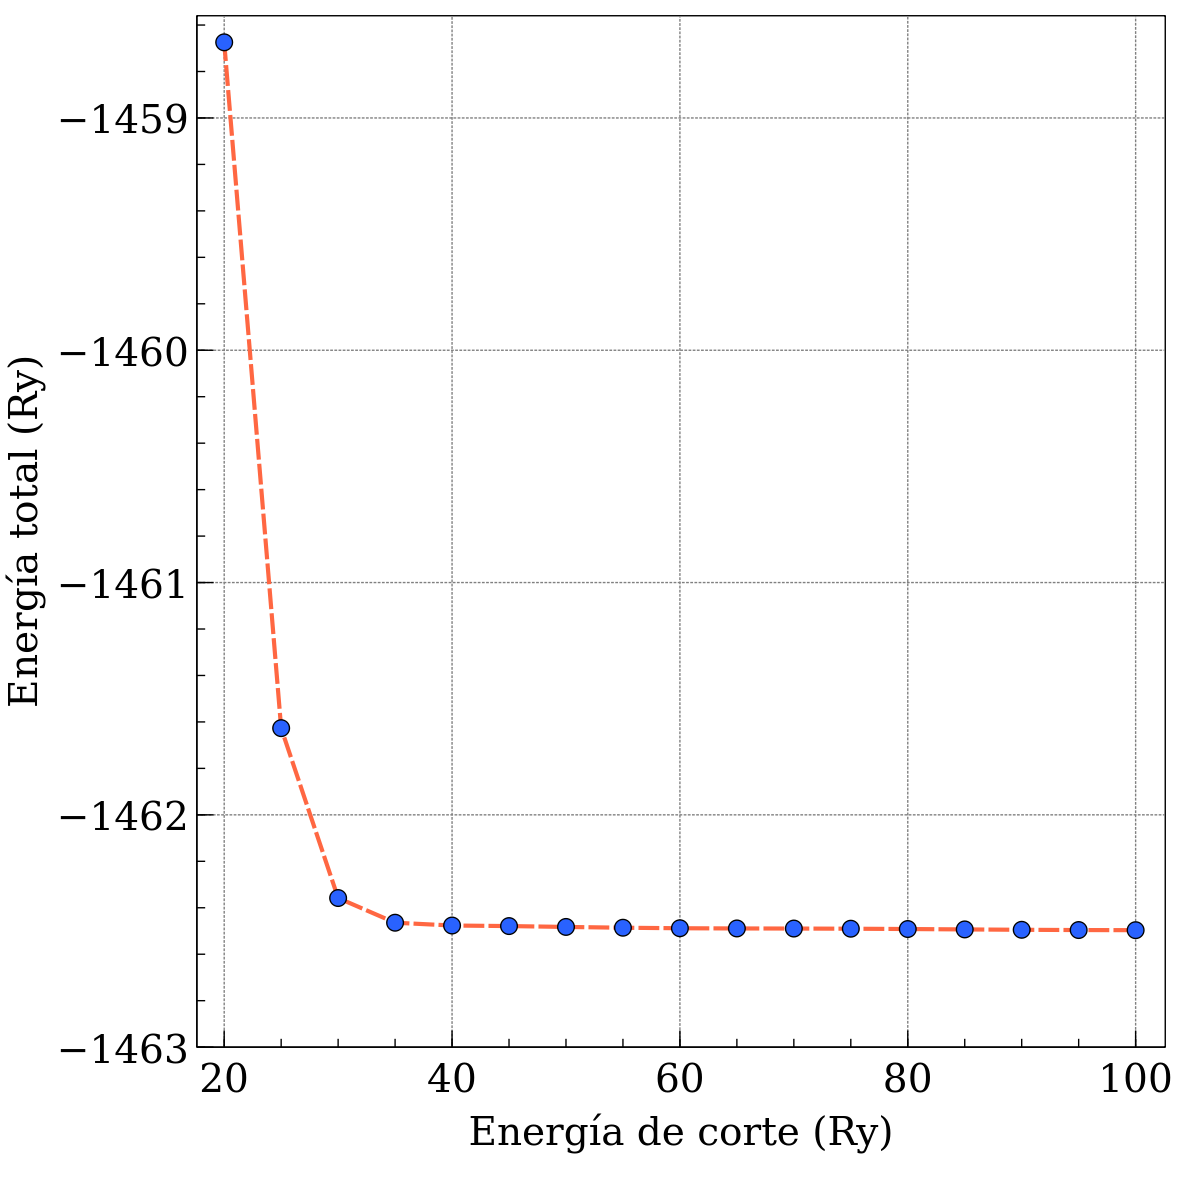
\includegraphics[width=1.0\textwidth]{contenido/resultados/img_resultados/energia_corte_YCO.png}
    \caption{Energ\'ia de corte para el $YCrO_{3}$}
\end{figure}
    \end{columns}
\end{frame}


\begin{frame}{Dimensi\'on de la grilla de puntos K}
        \begin{columns}[t]
            \column{0.5\textwidth}
\begin{figure}[H]
    \centering
    \includegraphics[width=1.0\textwidth]{contenido/resultados/img_resultados/energia_kp_BFO.png}
    \caption{Dimensi\'on de la grilla de puntos K para el $BiFeO_{3}$.}
\end{figure}
            \column{0.5\textwidth}
\begin{figure}[H]
    \centering
    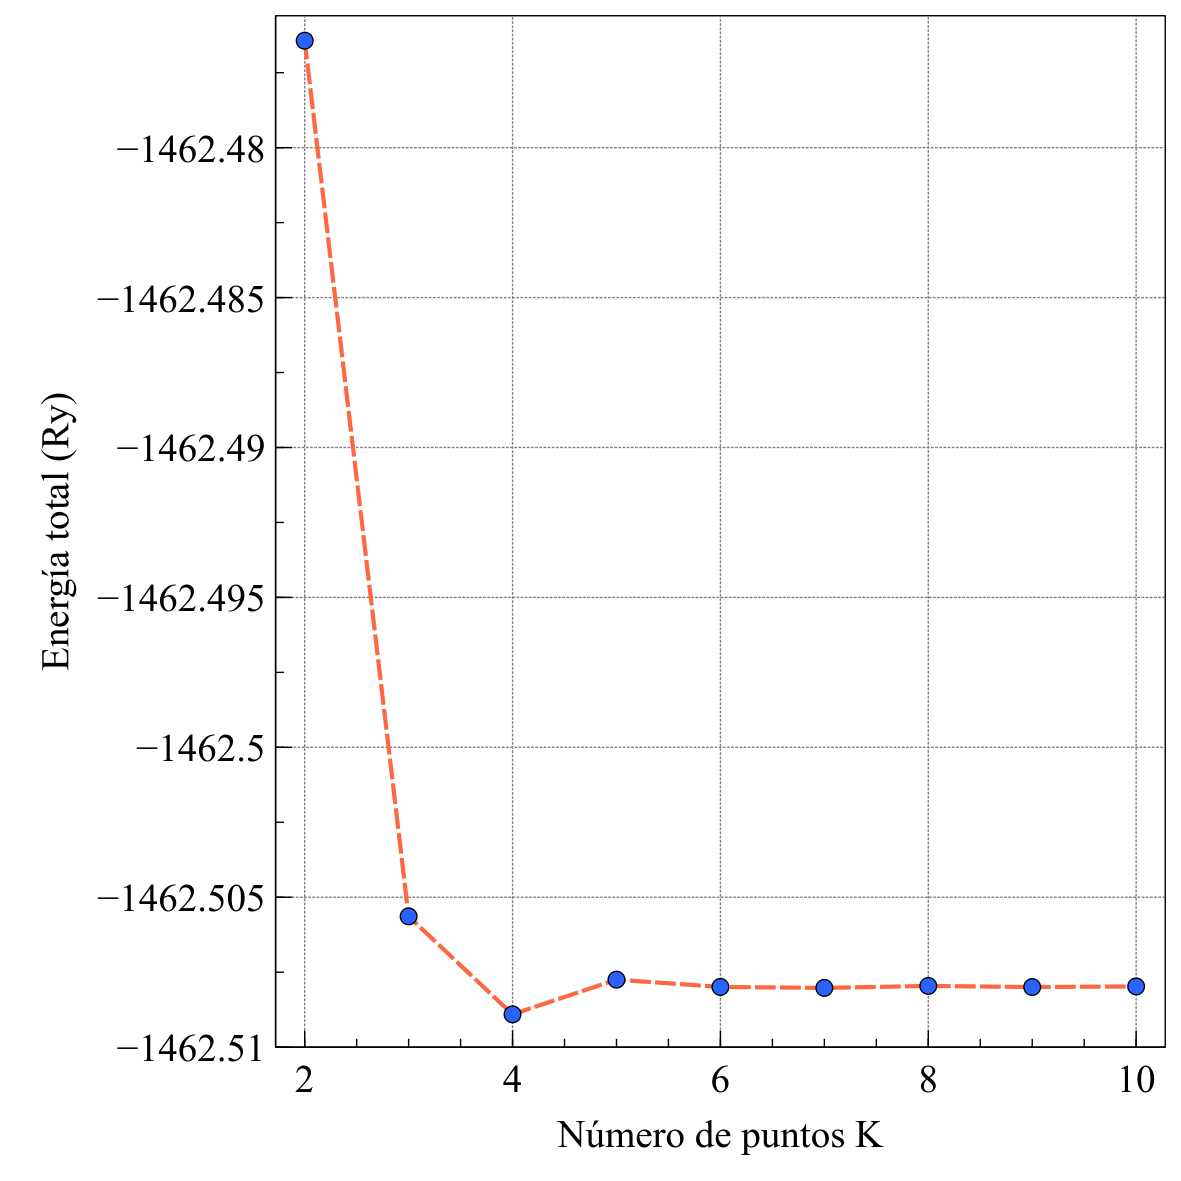
\includegraphics[width=1.0\textwidth]{contenido/resultados/img_resultados/energia_kp_YCO.png}
    \caption{Dimensi\'on de la grilla de puntos K para el $YCrO_{3}$.}
\end{figure}
        \end{columns}
\end{frame}

\subsection{Relajaci\'on de la estructura cristalina}
\begin{frame}{$BiFeO_{3}$ con arreglo antiferromagn\'etico tipo A}
            \begin{columns}[t]
        \column{0.5\textwidth}
        \begin{figure}[H]
            \centering
            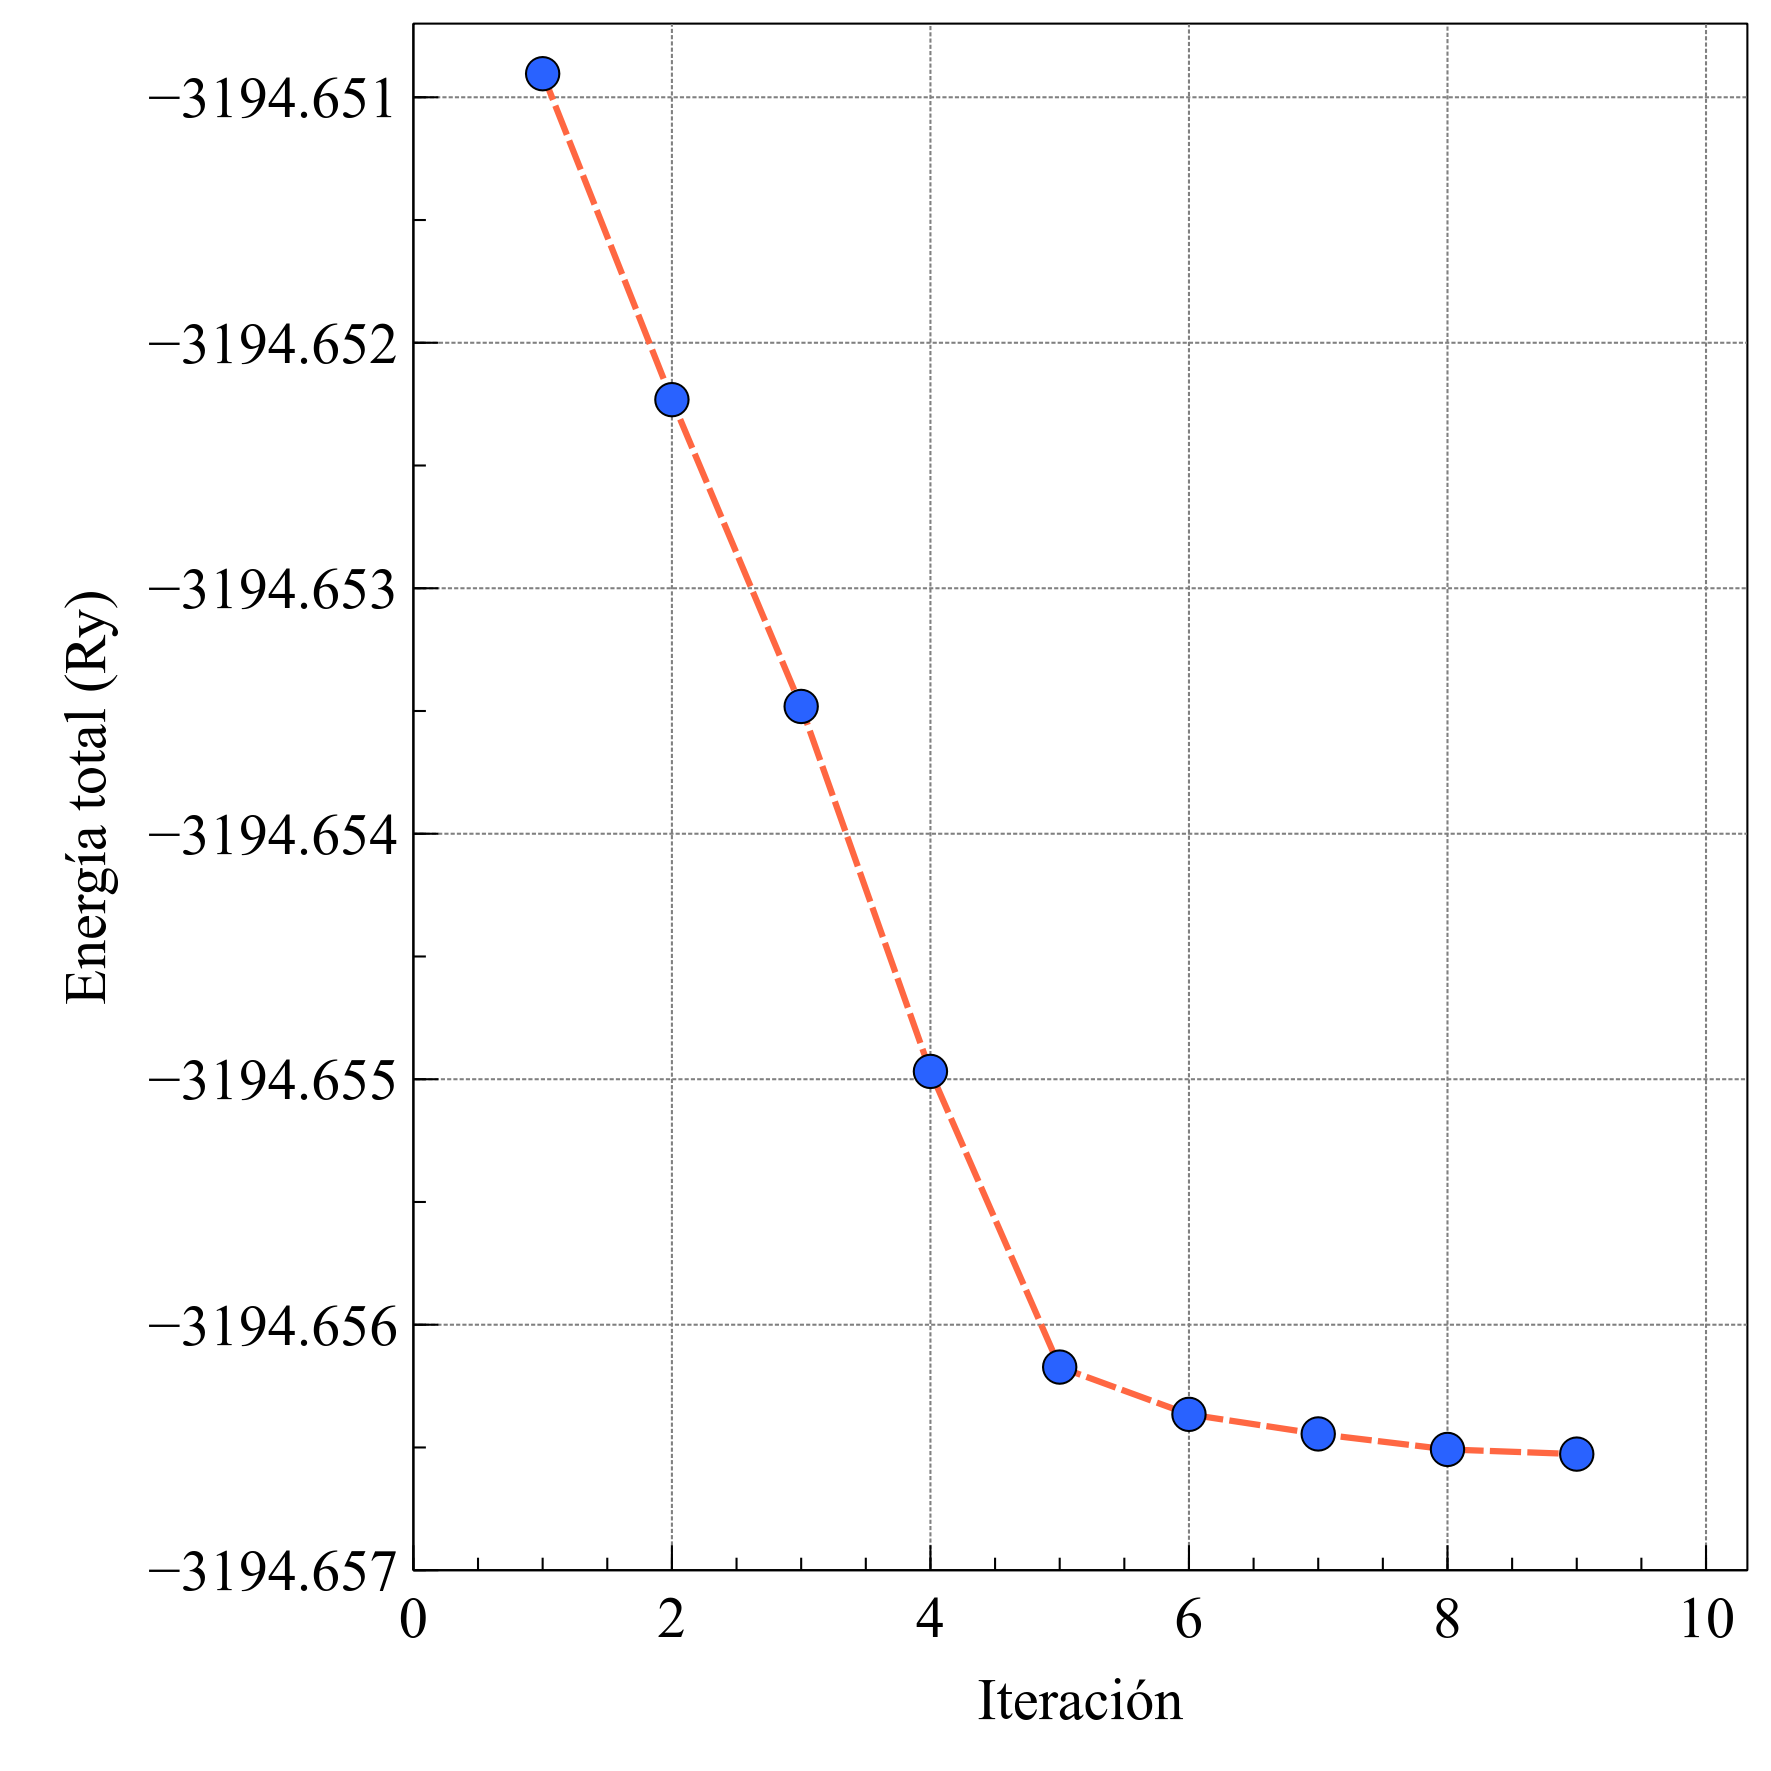
\includegraphics[width=0.9\textwidth]{contenido/resultados/img_resultados/energia_BFO_A.png}
            \caption{Minimizaci\'on de la energ\'ia del $BiFeO_{3}$ con arreglo 
                antiferromagn\'etico tipo A.}
        \end{figure}
        \column{0.5\textwidth}
        \begin{figure}[H]
            \centering
            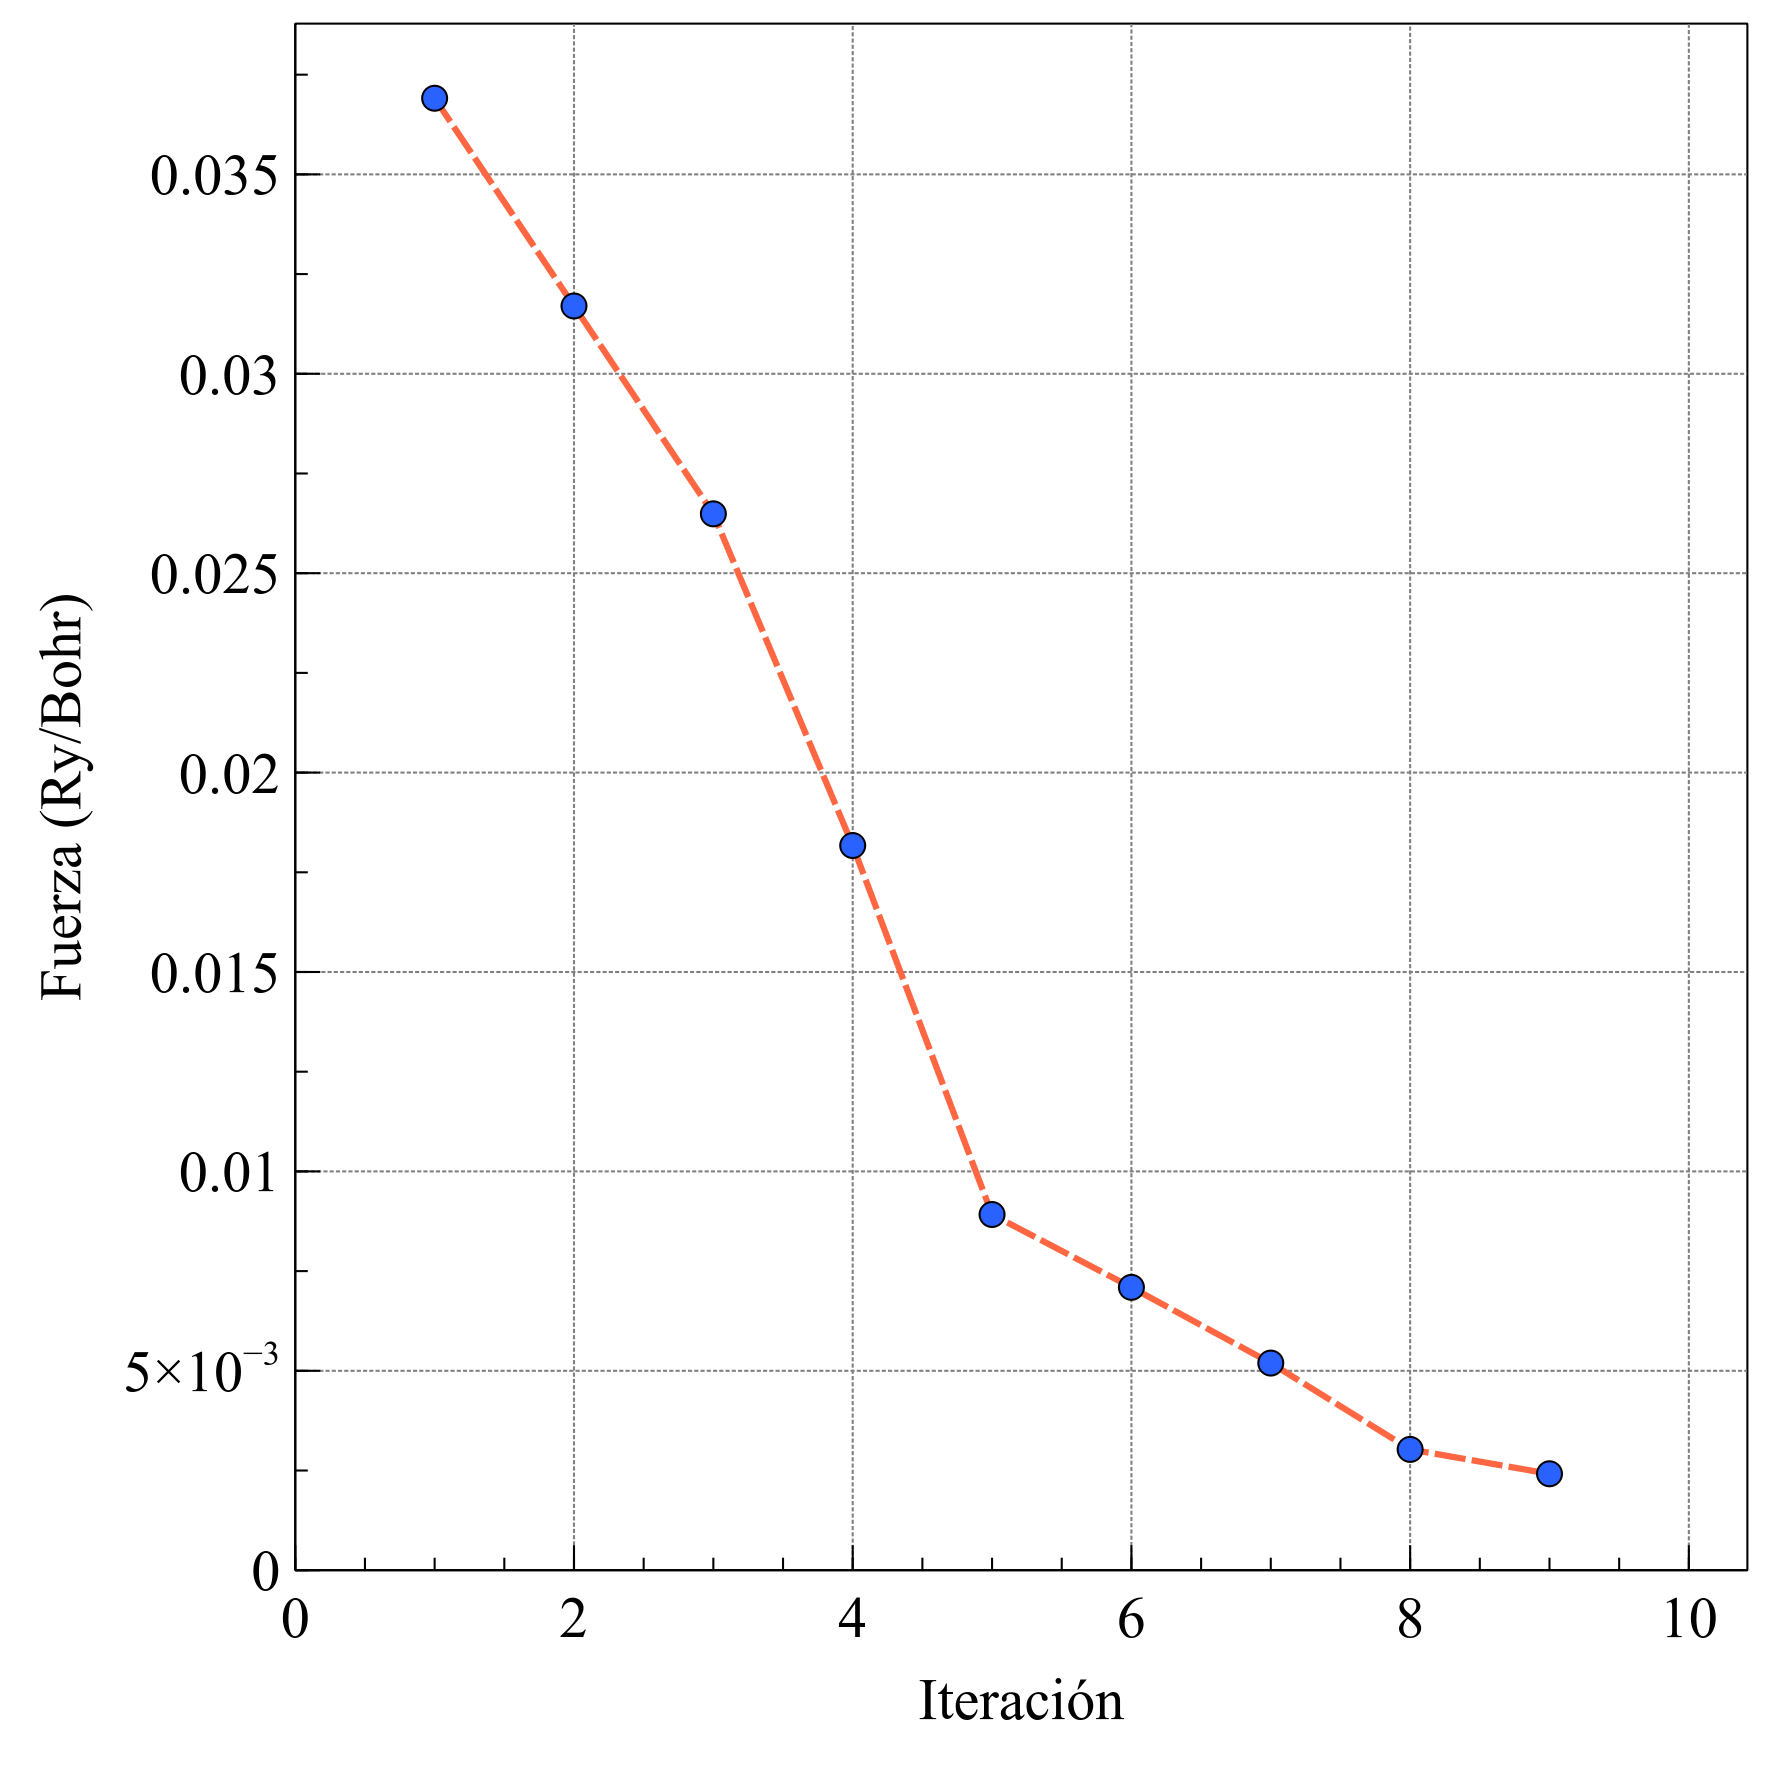
\includegraphics[width=0.9\textwidth]{contenido/resultados/img_resultados/fuerza_BFO_A.png}
            \caption{Minimizaci\'on de la fuerza del $BiFeO_{3}$ con arreglo 
            antiferromagn\'etico tipo A.}
        \end{figure}
    \end{columns}
\centering
\textbf{El sistema converge luego de 9 iteraciones.}
\end{frame}


\begin{frame}{$BiFeO_{3}$ con arreglo antiferromagn\'etico tipo G}
    \begin{columns}[t]
        \column{0.5\textwidth}
        \begin{figure}[H]
            \centering
            \includegraphics[width=0.9\textwidth]{contenido/resultados/img_resultados/energia_BFO_G.png}
            \caption{Minimizaci\'on de la energ\'ia del $BiFeO_{3}$ con arreglo 
                antiferromagn\'etico tipo G.}
        \end{figure}
        \column{0.5\textwidth}
        \begin{figure}[H]
            \centering
            \includegraphics[width=0.9\textwidth]{contenido/resultados/img_resultados/fuerza_BFO_G.png}
            \caption{Minimizaci\'on de la fuerza del $BiFeO_{3}$ con arreglo 
                antiferromagn\'etico tipo G.}
        \end{figure}
    \end{columns}
\centering
\textbf{El sistema converge luego de 9 iteraciones.}
\end{frame}


\begin{frame}{$YCrO_{3}$ con arreglo antiferromagn\'etico tipo A}
    \begin{columns}[t]
        \column{0.5\textwidth}
        \begin{figure}[H]
            \centering
            \includegraphics[width=0.9\textwidth]{contenido/resultados/img_resultados/energia_YCO_A.png}
            \caption{Minimizaci\'on de la energ\'ia del $YCrO_{3}$ con arreglo 
                antiferromagn\'etico tipo A.}
        \end{figure}
        \column{0.5\textwidth}
        \begin{figure}[H]
            \centering
            \includegraphics[width=0.9\textwidth]{contenido/resultados/img_resultados/fuerza_YCO_A.png}
            \caption{Minimizaci\'on de la fuerza del $YCrO_{3}$ con arreglo 
                antiferromagn\'etico tipo A.}
        \end{figure}
    \end{columns}
\centering
\textbf{El sistema converge luego de 14 iteraciones.}
\end{frame}


\begin{frame}{$YCrO_{3}$ con arreglo antiferromagn\'etico tipo C}
    \begin{columns}[t]
        \column{0.5\textwidth}
        \begin{figure}[H]
            \centering
            \includegraphics[width=0.9\textwidth]{contenido/resultados/img_resultados/energia_YCO_C.png}
            \caption{Minimizaci\'on de la energ\'ia del $YCrO_{3}$ con arreglo 
                antiferromagn\'etico tipo C.}
        \end{figure}
        \column{0.5\textwidth}
        \begin{figure}[H]
            \centering
            \includegraphics[width=0.9\textwidth]{contenido/resultados/img_resultados/fuerza_YCO_C.png}
            \caption{Minimizaci\'on de la fuerza del $YCrO_{3}$ con arreglo 
                antiferromagn\'etico tipo C.}
        \end{figure}
    \end{columns}
\centering
\textbf{El sistema converge luego de 12 iteraciones.}
\end{frame}


\begin{frame}{$YCrO_{3}$ con arreglo antiferromagn\'etico tipo G}
    \begin{columns}[t]
        \column{0.5\textwidth}
        \begin{figure}[H]
            \centering
            \includegraphics[width=0.9\textwidth]{contenido/resultados/img_resultados/energia_YCO_G.png}
            \caption{Minimizaci\'on de la energ\'ia del $YCrO_{3}$ con arreglo 
                antiferromagn\'etico tipo G.}
        \end{figure}
        \column{0.5\textwidth}
        \begin{figure}[H]
            \centering
            \includegraphics[width=0.9\textwidth]{contenido/resultados/img_resultados/fuerza_YCO_G.png}
            \caption{Minimizaci\'on de la fuerza del $YCrO_{3}$ con arreglo 
                antiferromagn\'etico tipo G.}
        \end{figure}
    \end{columns}
\centering
\textbf{El sistema converge luego de 13 iteraciones.}
\end{frame}

\subsection{Bandas de energ\'ia y densidades de estado}
\begin{frame}{Estructura de bandas del $BiFeO_{3}$}
\begin{columns}[t]
    \column{0.5\textwidth}
    \begin{figure}[H]
        \centering
        \includegraphics[width=1.0\textwidth]{contenido/resultados/img_resultados/BFO_bandas_A.png}
        \caption{Bandas de energ\'ia del $BiFeO_{3}$ con arreglo         
        antiferromagn\'etico tipo A.}
    \end{figure}
\centering
\textbf{Gap: $1.4$ eV.}
    \column{0.5\textwidth}
    \begin{figure}[H]
        \centering
        \includegraphics[width=1.0\textwidth]{contenido/resultados/img_resultados/BFO_bandas_G.png}
        \caption{Bandas de energ\'ia del $BiFeO_{3}$ con arreglo 
            antiferromagn\'etico tipo G.}
    \end{figure}
\centering
\textbf{Gap: $1.8$ eV.} \\
{\scriptsize 1.9 eV. S. Ju et al. Chem. Phys. 130, 2009 } \\
{\scriptsize 1.8 eV Zait Ayala Tesis maestr\'ia. }
\end{columns}    
\end{frame}

\begin{frame}{Densidad de estados del $BiFeO_{3}$}
\begin{columns}[t]
    \column{0.5\textwidth}
    \begin{figure}[H]
        \centering
        \includegraphics[width=1.0\textwidth]{contenido/resultados/img_resultados/BFO_DOS_A.png}
        \caption{Densidad de estados total del $BiFeO_{3}$ con arreglo         
            antiferromagn\'etico tipo A.}
    \end{figure}
    \column{0.5\textwidth}
    \begin{figure}[H]
        \centering
        \includegraphics[width=1.0\textwidth]{contenido/resultados/img_resultados/BFO_DOS_G.png}
        \caption{Densidad de estados total del $BiFeO_{3}$ con arreglo 
            antiferromagn\'etico tipo G.}
    \end{figure}
\end{columns}           
\end{frame}

\begin{frame}
    \begin{columns}[t]
        \column{0.5\textwidth}
        \begin{figure}[H]
            \centering
            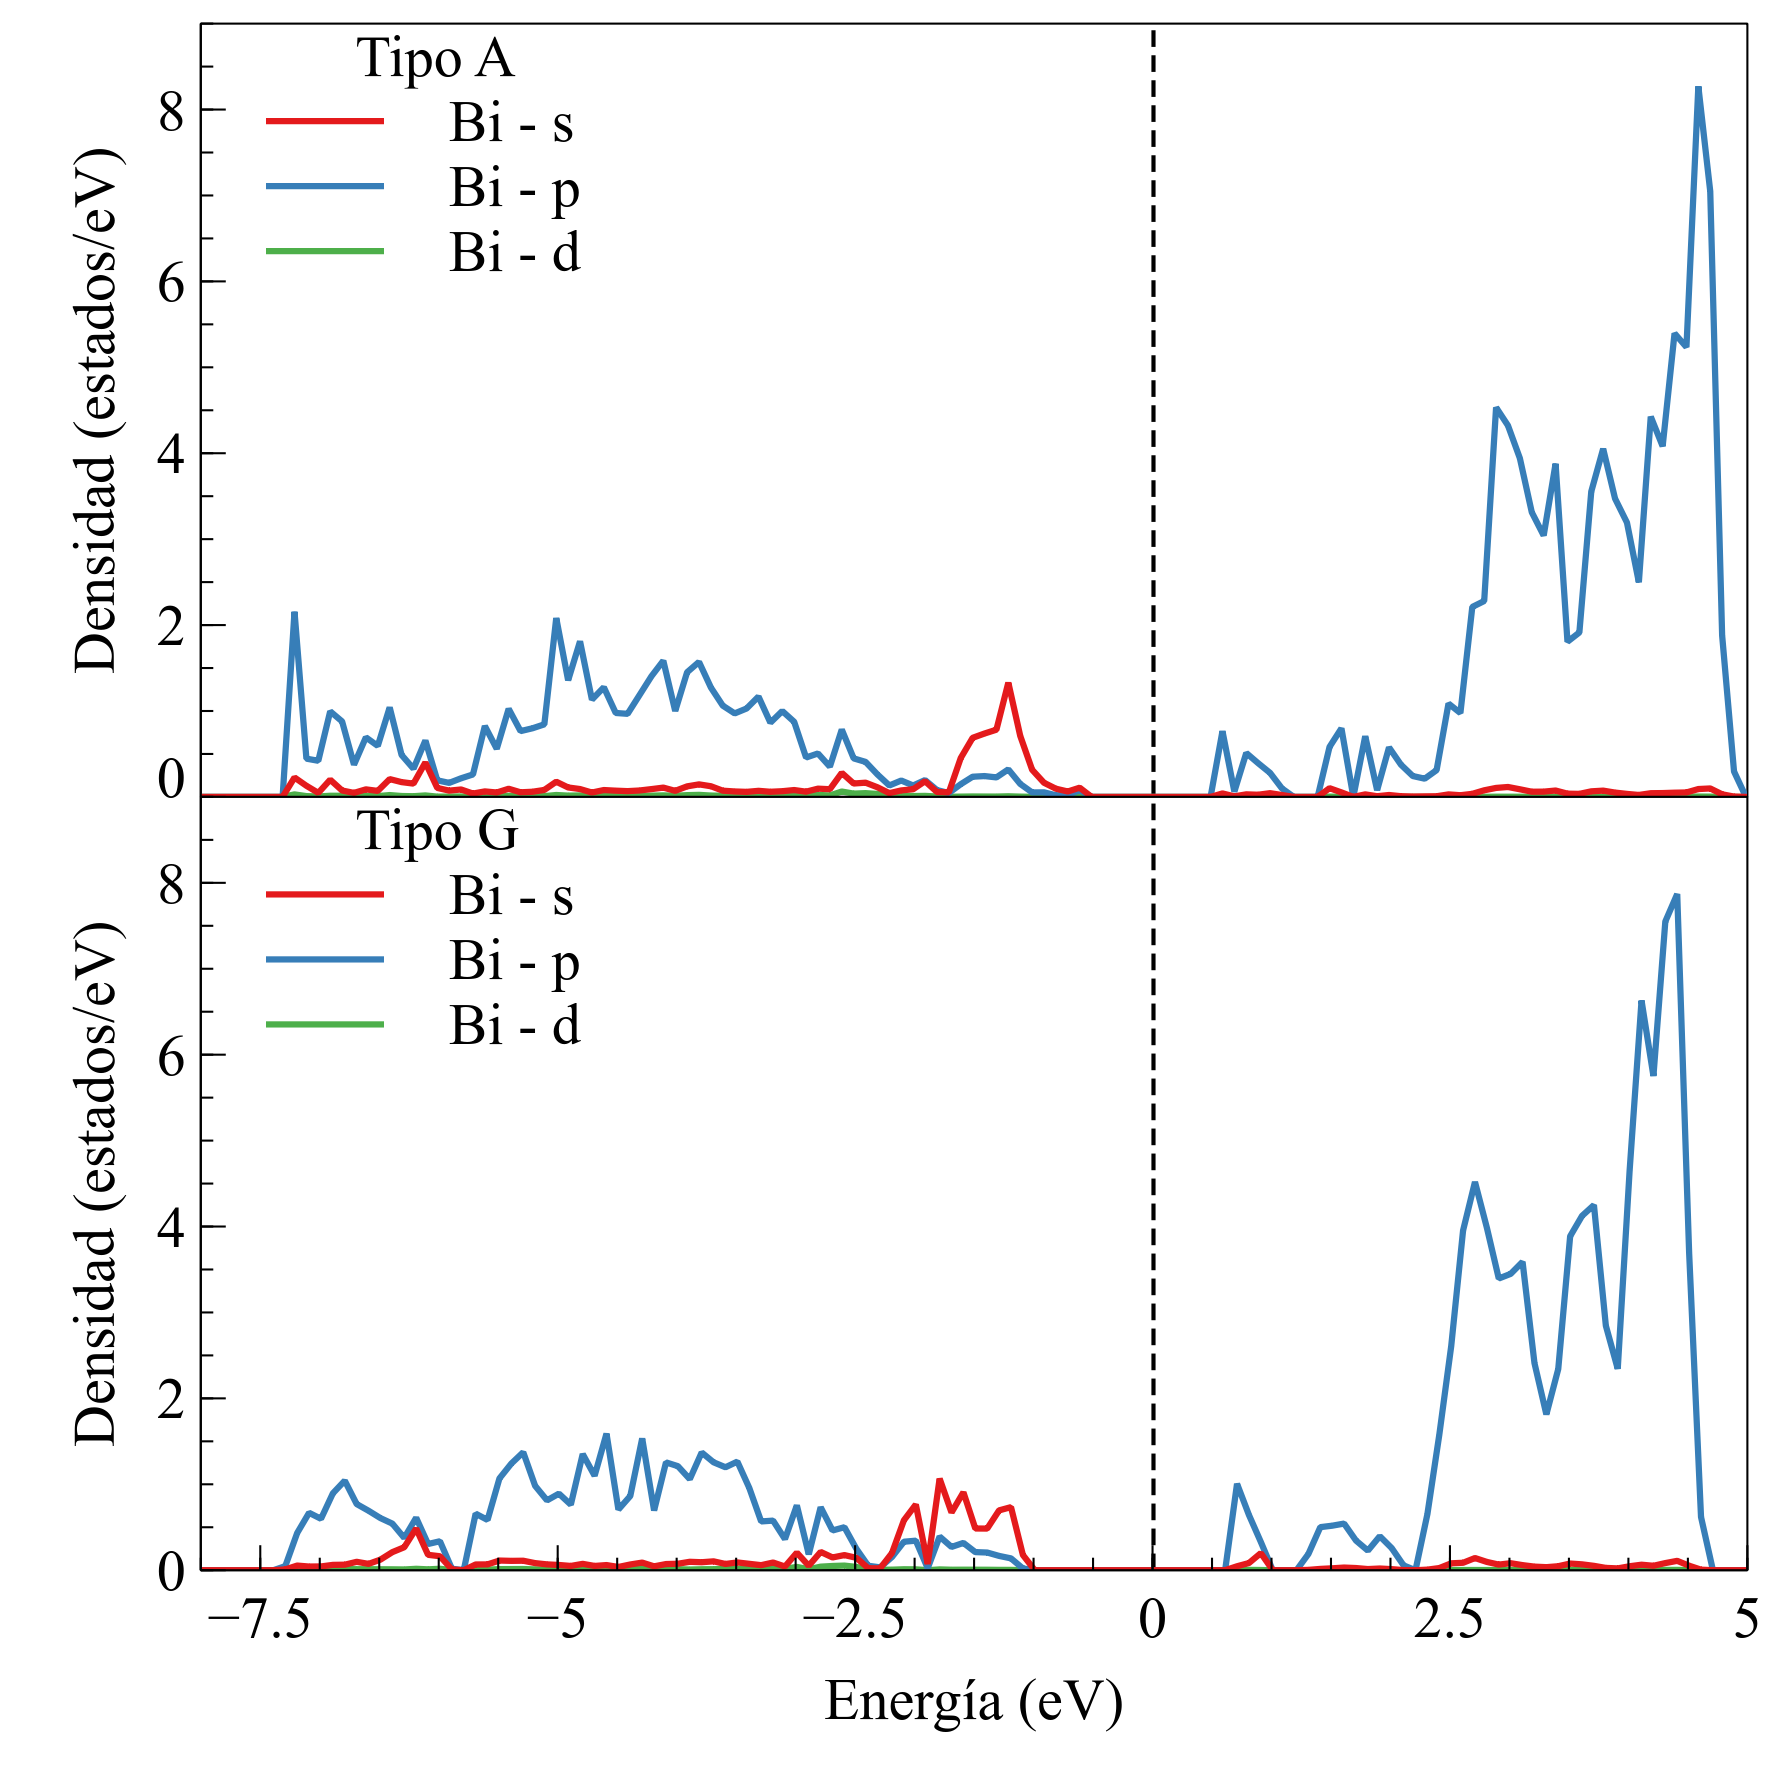
\includegraphics[width=1.0\textwidth]{contenido/resultados/img_resultados/BFO_Bi_tipos.png}
            \caption{Densidad de estados parcial del bismuto del $BiFeO_{3}$.}
        \end{figure}
        \column{0.5\textwidth}
        \begin{figure}[H]
            \centering
            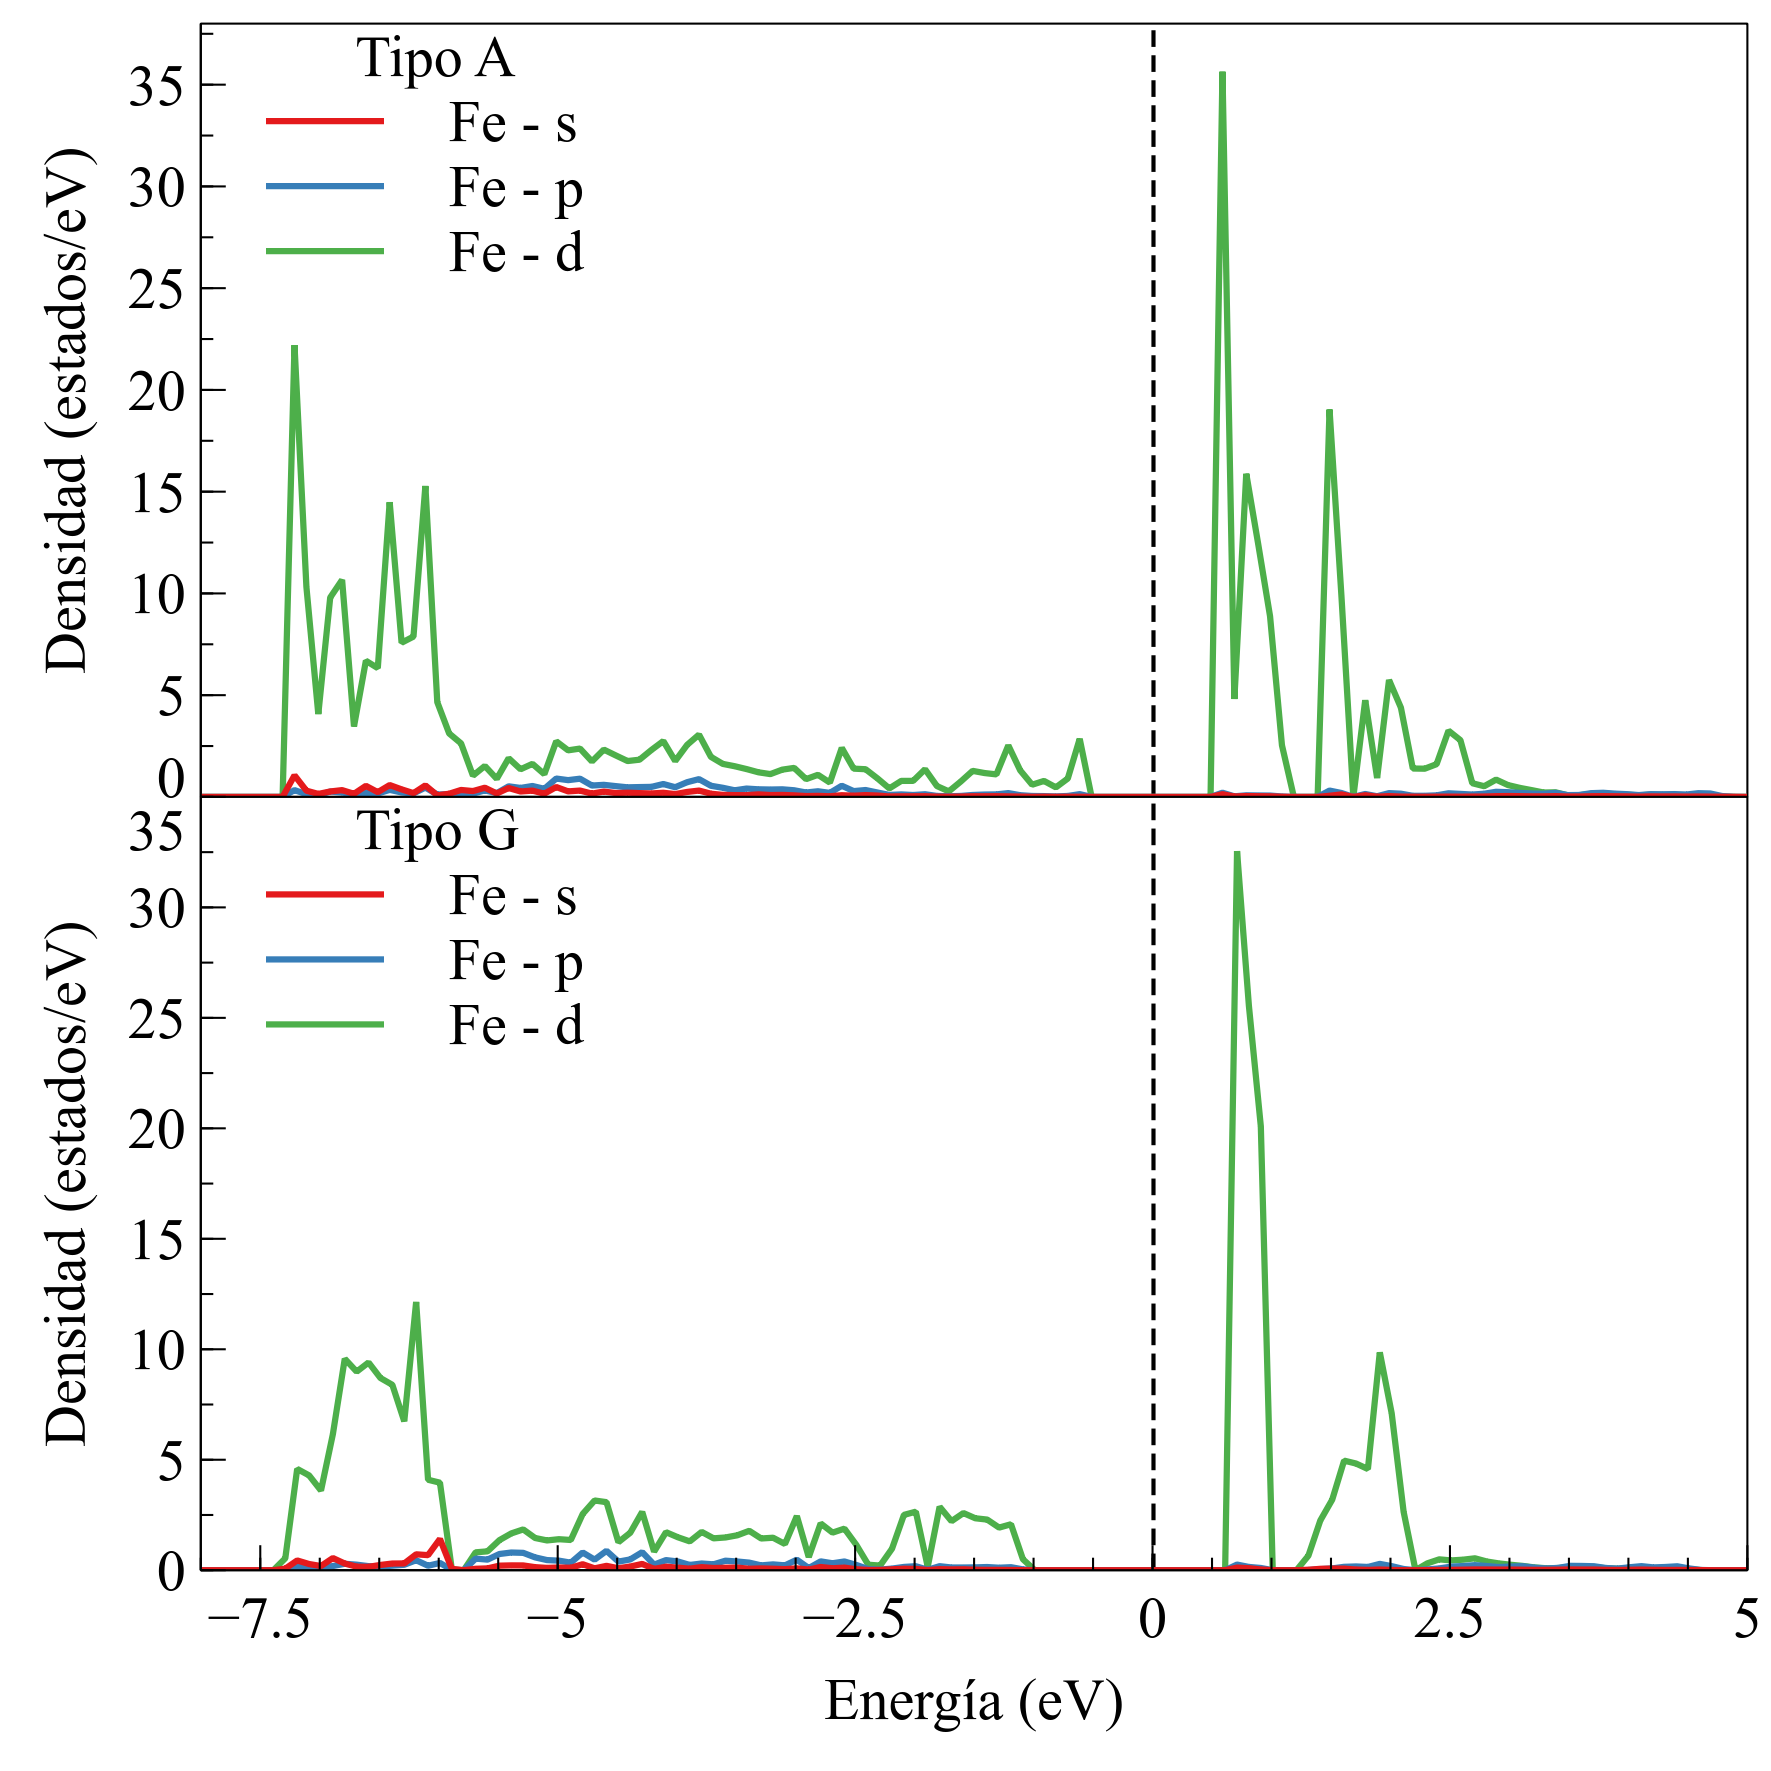
\includegraphics[width=1.0\textwidth]{contenido/resultados/img_resultados/BFO_Fe_tipos.png}
            \caption{Densidad de estados parcial del hierro del $BiFeO_{3}$.}
        \end{figure}
    \end{columns}
\end{frame}

\begin{frame}
     \begin{figure}[H]
        \centering
        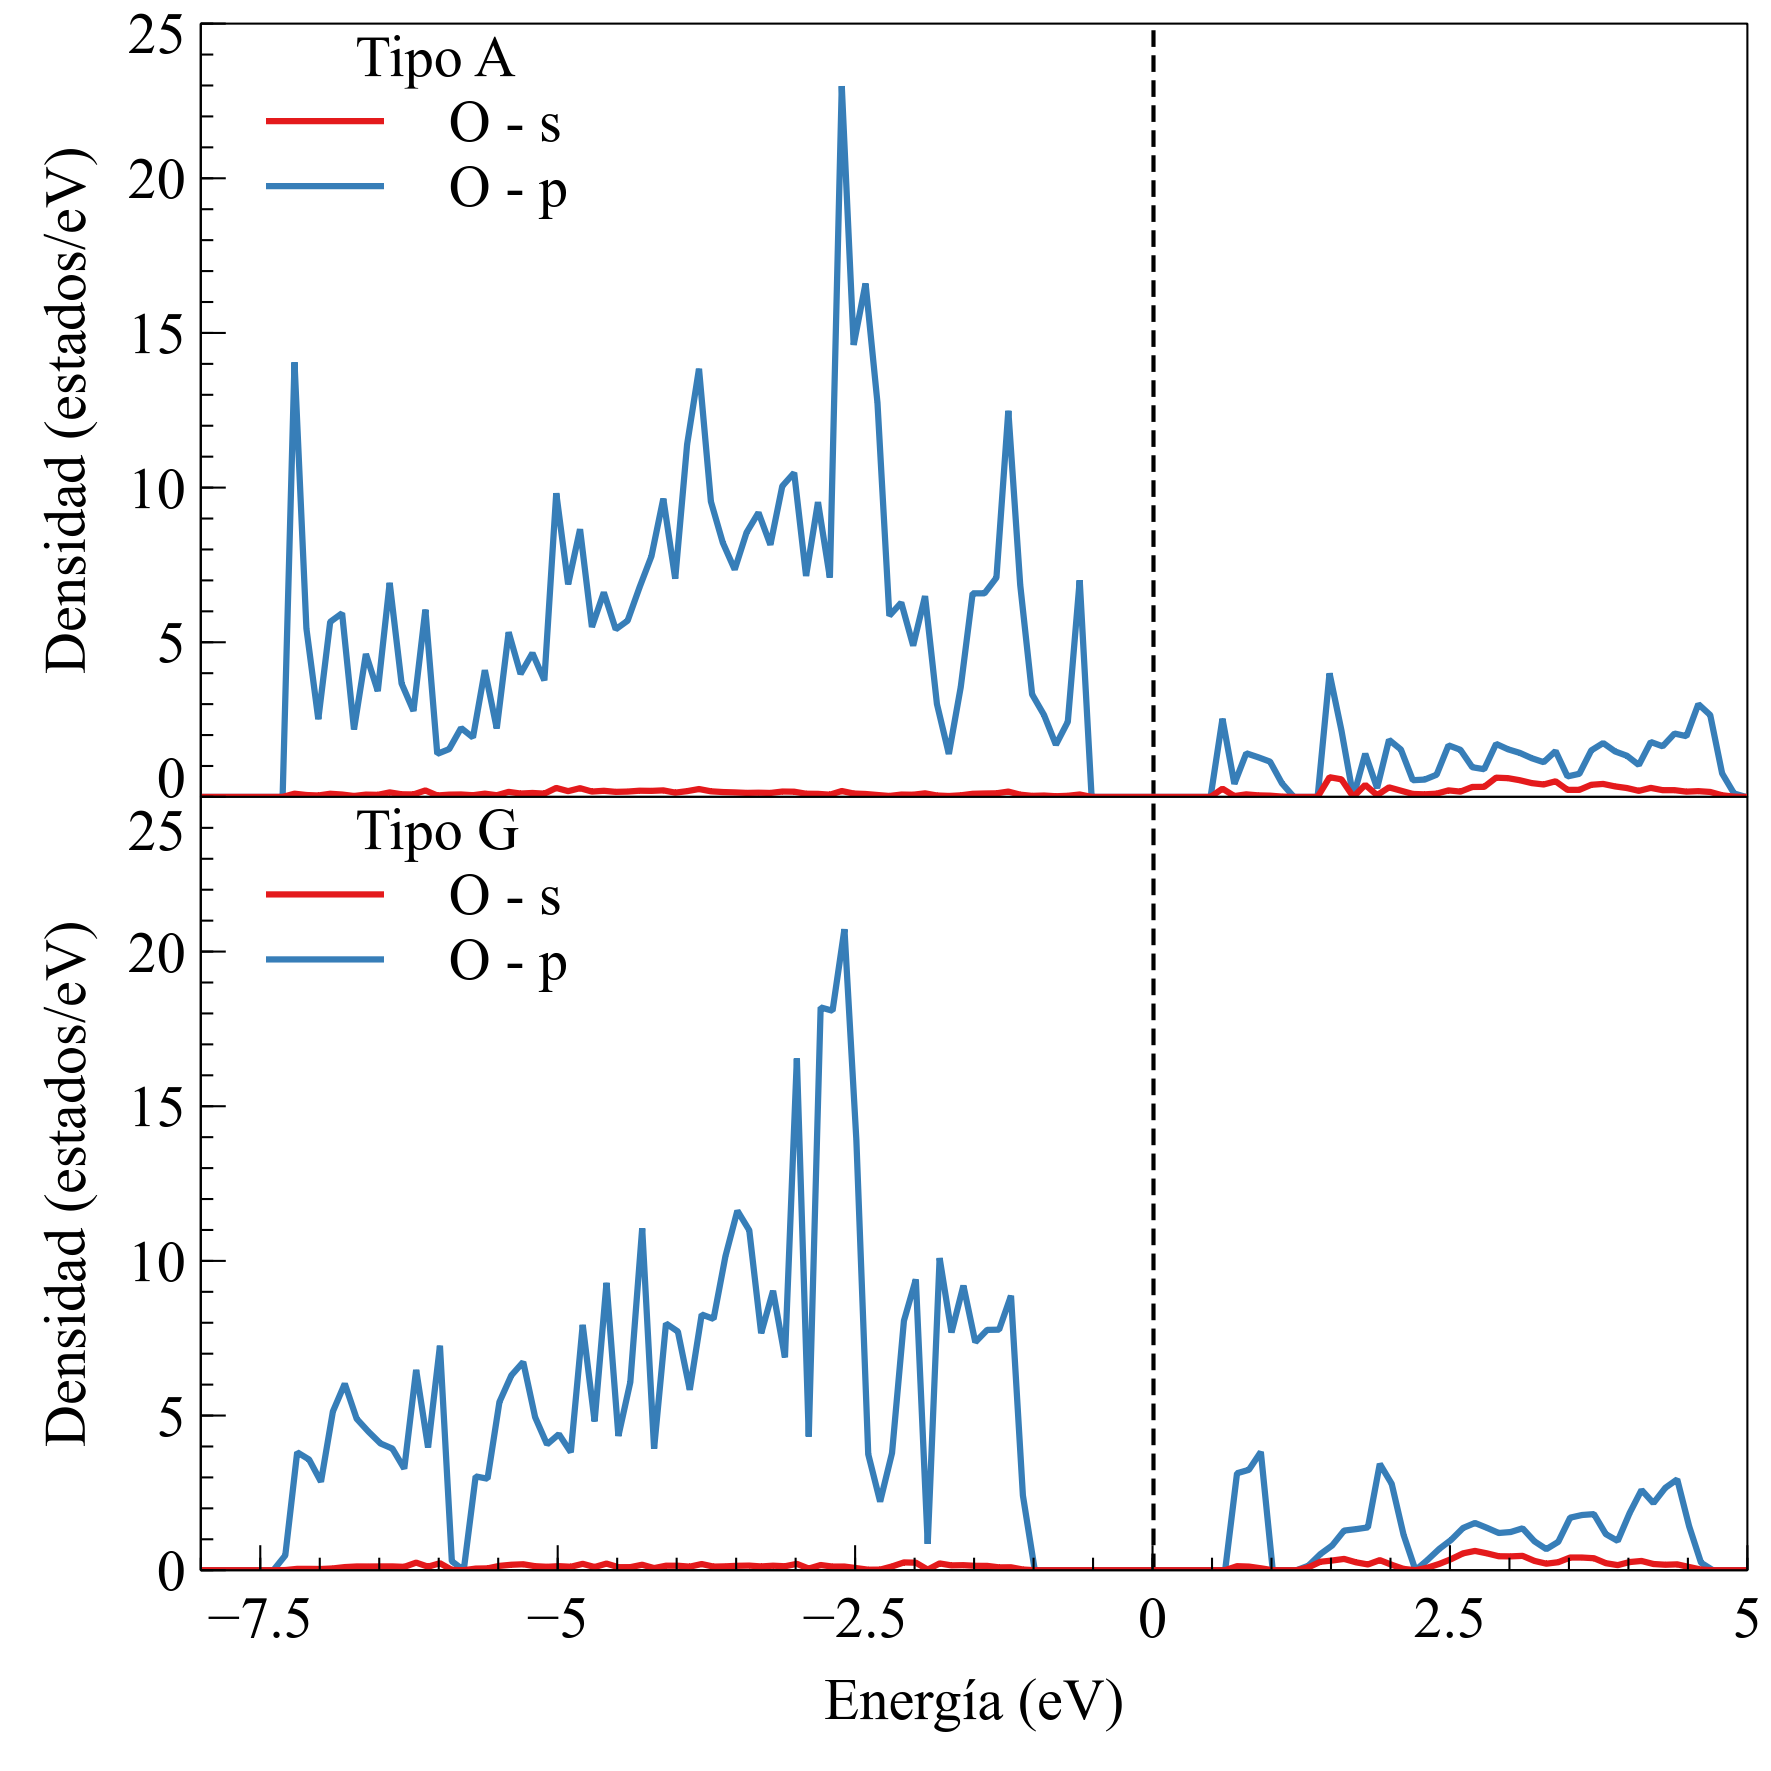
\includegraphics[width=0.5\textwidth]{contenido/resultados/img_resultados/BFO_O_tipos.png}
        \caption{Densidad de estados parcial del ox\'igeno del $BiFeO_{3}$.}
    \end{figure}
\end{frame}
\begin{frame}{Estructura de bandas del $YCrO_{3}$}
    \begin{columns}[t]
        \column{0.5\textwidth}
        \begin{figure}[H]
            \centering
            \includegraphics[width=1.0\textwidth]{contenido/resultados/img_resultados/YCO_bandas_A.png}
            \caption{Bandas de energ\'ia del $YCrO_{3}$ con arreglo         
                antiferromagn\'etico tipo A.}
        \end{figure}
        \centering
        \textbf{Gap: $1.3$ eV.}
        \column{0.5\textwidth}
        \begin{figure}[H]
            \centering
            \includegraphics[width=1.0\textwidth]{contenido/resultados/img_resultados/YCO_bandas_C.png}
            \caption{Bandas de energ\'ia del $YCrO_{3}$ con arreglo 
                antiferromagn\'etico tipo C.}
        \end{figure}
        \centering
        \textbf{Gap: $1.32$ eV.}
    \end{columns}
\end{frame}

\begin{frame}
    \begin{figure}[H]
        \centering
        \includegraphics[width=0.5\textwidth]{contenido/resultados/img_resultados/YCO_bandas_G.png}
        \caption{Bandas de energ\'ia del $YCrO_{3}$ con arreglo 
            antiferromagn\'etico tipo G.}
    \end{figure}
    \centering
    \textbf{Gap: $1.6$ eV.} \\
    {\scriptsize 1.8 eV. Serrao et al. Physical Review B, 72, 2005 }
\end{frame}

\begin{frame}{Densidad de estados del $YCrO_{3}$}
\begin{columns}[t]
    \column{0.5\textwidth}
    \begin{figure}[H]
        \centering
        \includegraphics[width=1.0\textwidth]{contenido/resultados/img_resultados/YCO_DOS_A.png}
        \caption{Densidad de estados total del $YCrO_{3}$ con arreglo         
            antiferromagn\'etico tipo A.}
    \end{figure}
    \column{0.5\textwidth}
    \begin{figure}[H]
        \centering
        \includegraphics[width=1.0\textwidth]{contenido/resultados/img_resultados/YCO_DOS_C.png}
        \caption{Densidad de estados total del $YCrO_{3}$ con arreglo 
            antiferromagn\'etico tipo C.}
    \end{figure}
\end{columns} 
\end{frame}

\begin{frame}
\begin{figure}[H]
    \centering
    \includegraphics[width=0.5\textwidth]{contenido/resultados/img_resultados/YCO_DOS_G.png}
    \caption{Densidad de estados total del $YCrO_{3}$ con arreglo 
        antiferromagn\'etico tipo G.}
\end{figure}
\end{frame}

\begin{frame}
\begin{columns}[t]
    \column{0.5\textwidth}
    \begin{figure}[H]
        \centering
        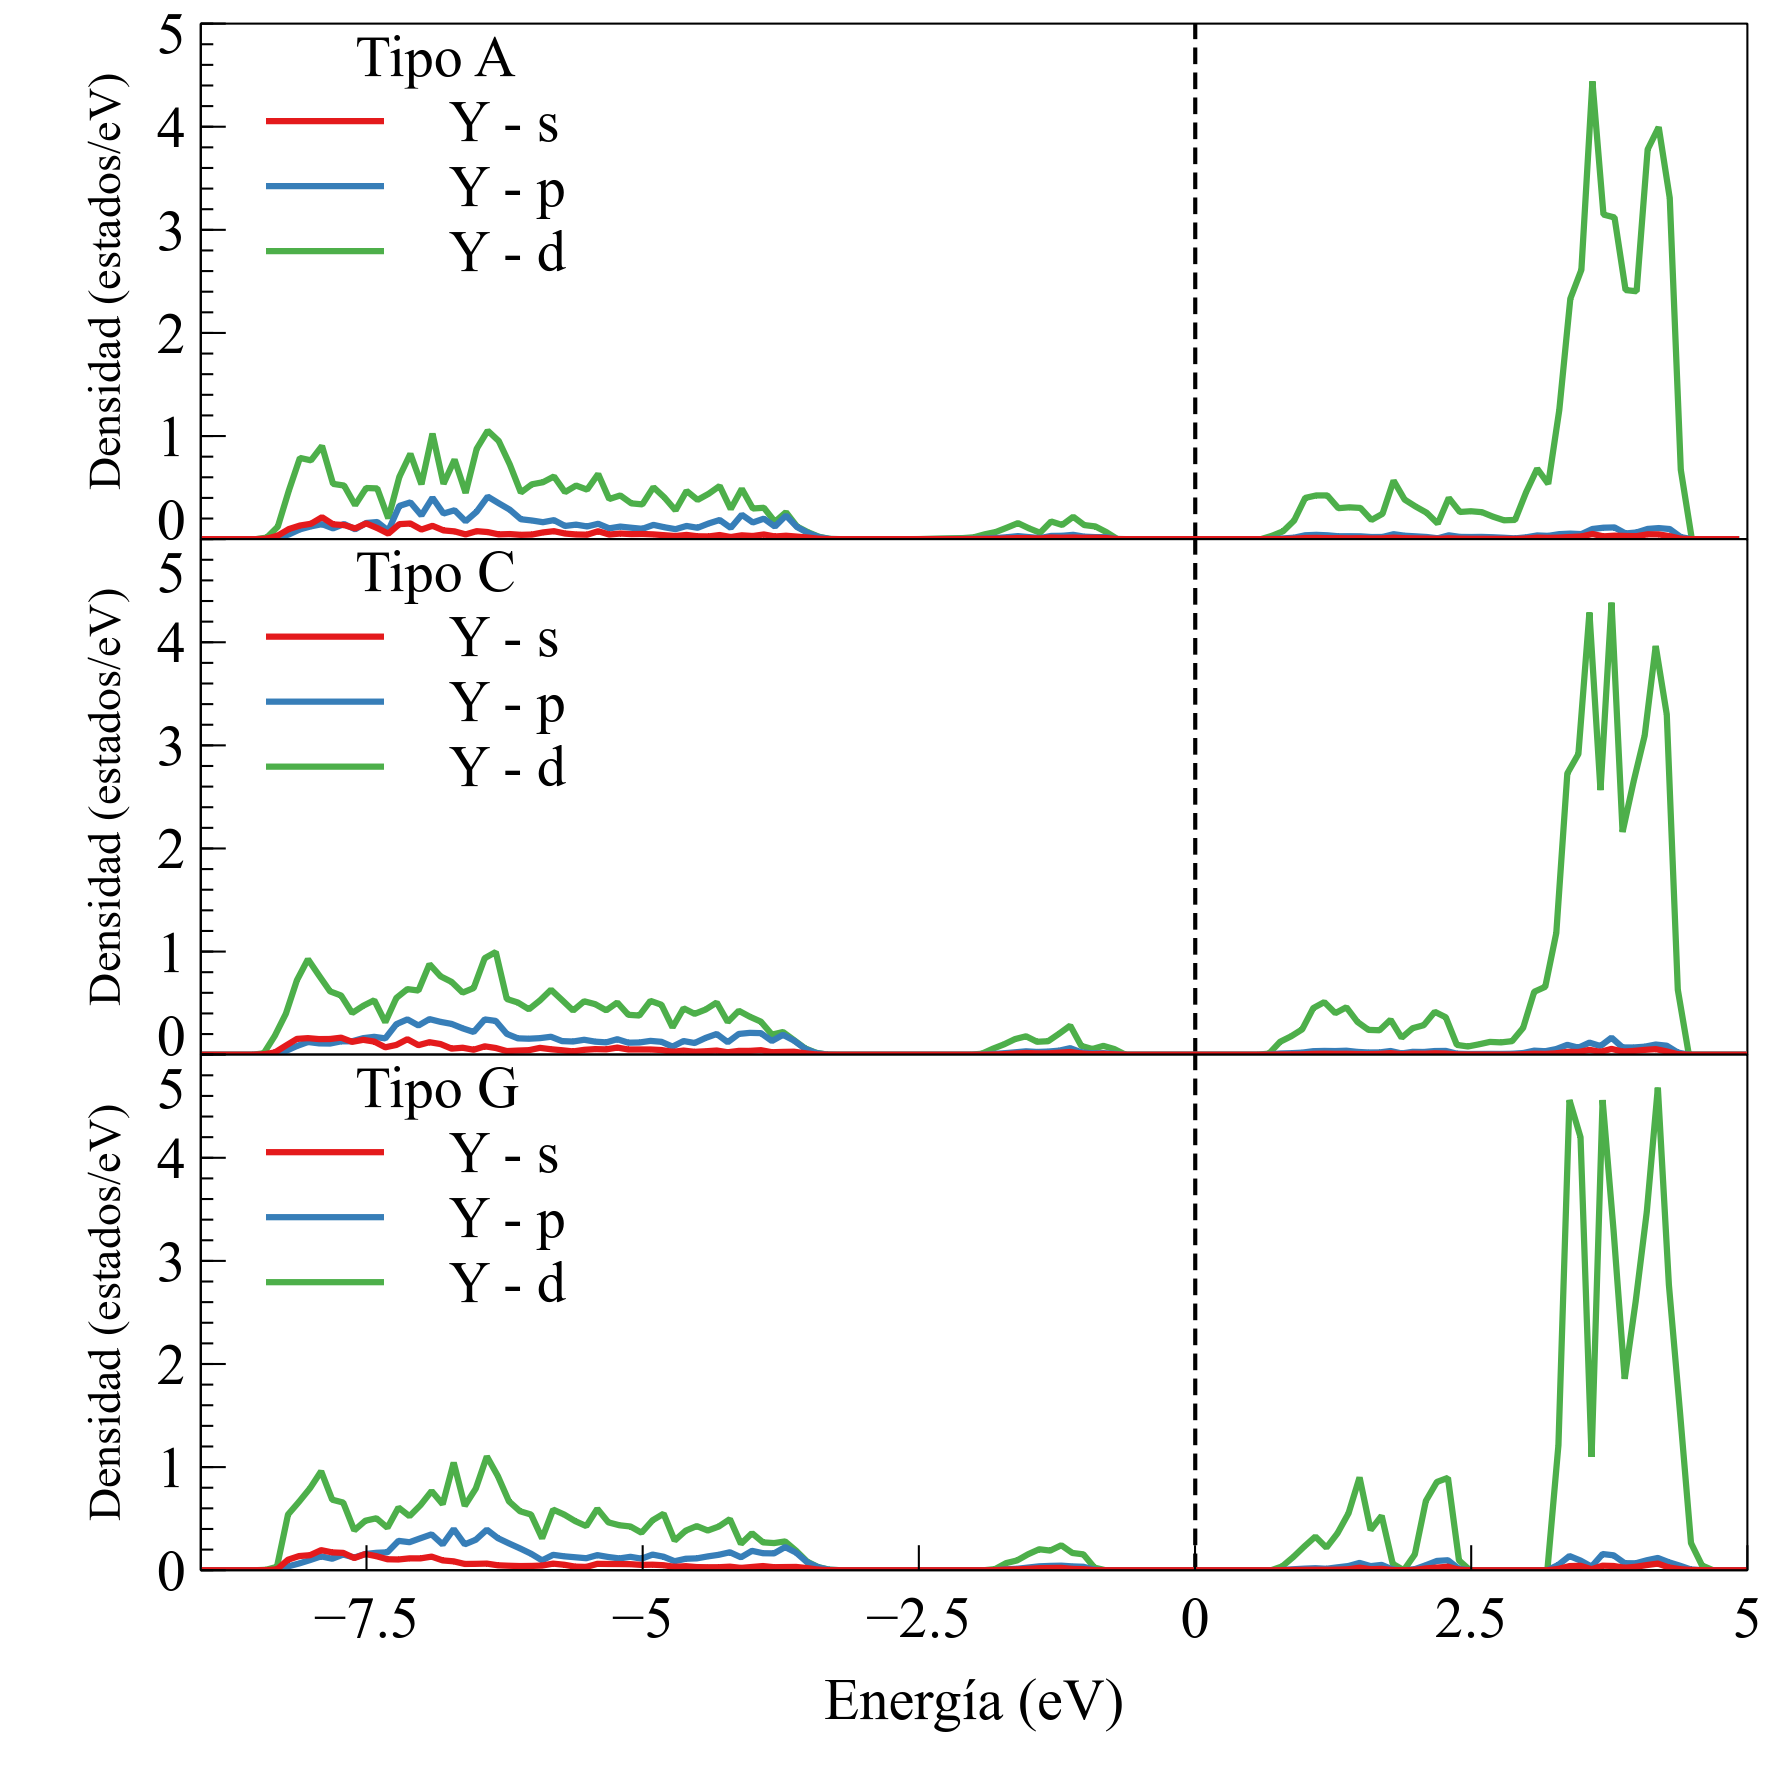
\includegraphics[width=1.0\textwidth]{contenido/resultados/img_resultados/YCO_Y_tipos.png}
        \caption{Densidad de estados parcial del itrio del $YCrO_{3}$.}
    \end{figure}
    \column{0.5\textwidth}
    \begin{figure}[H]
        \centering
        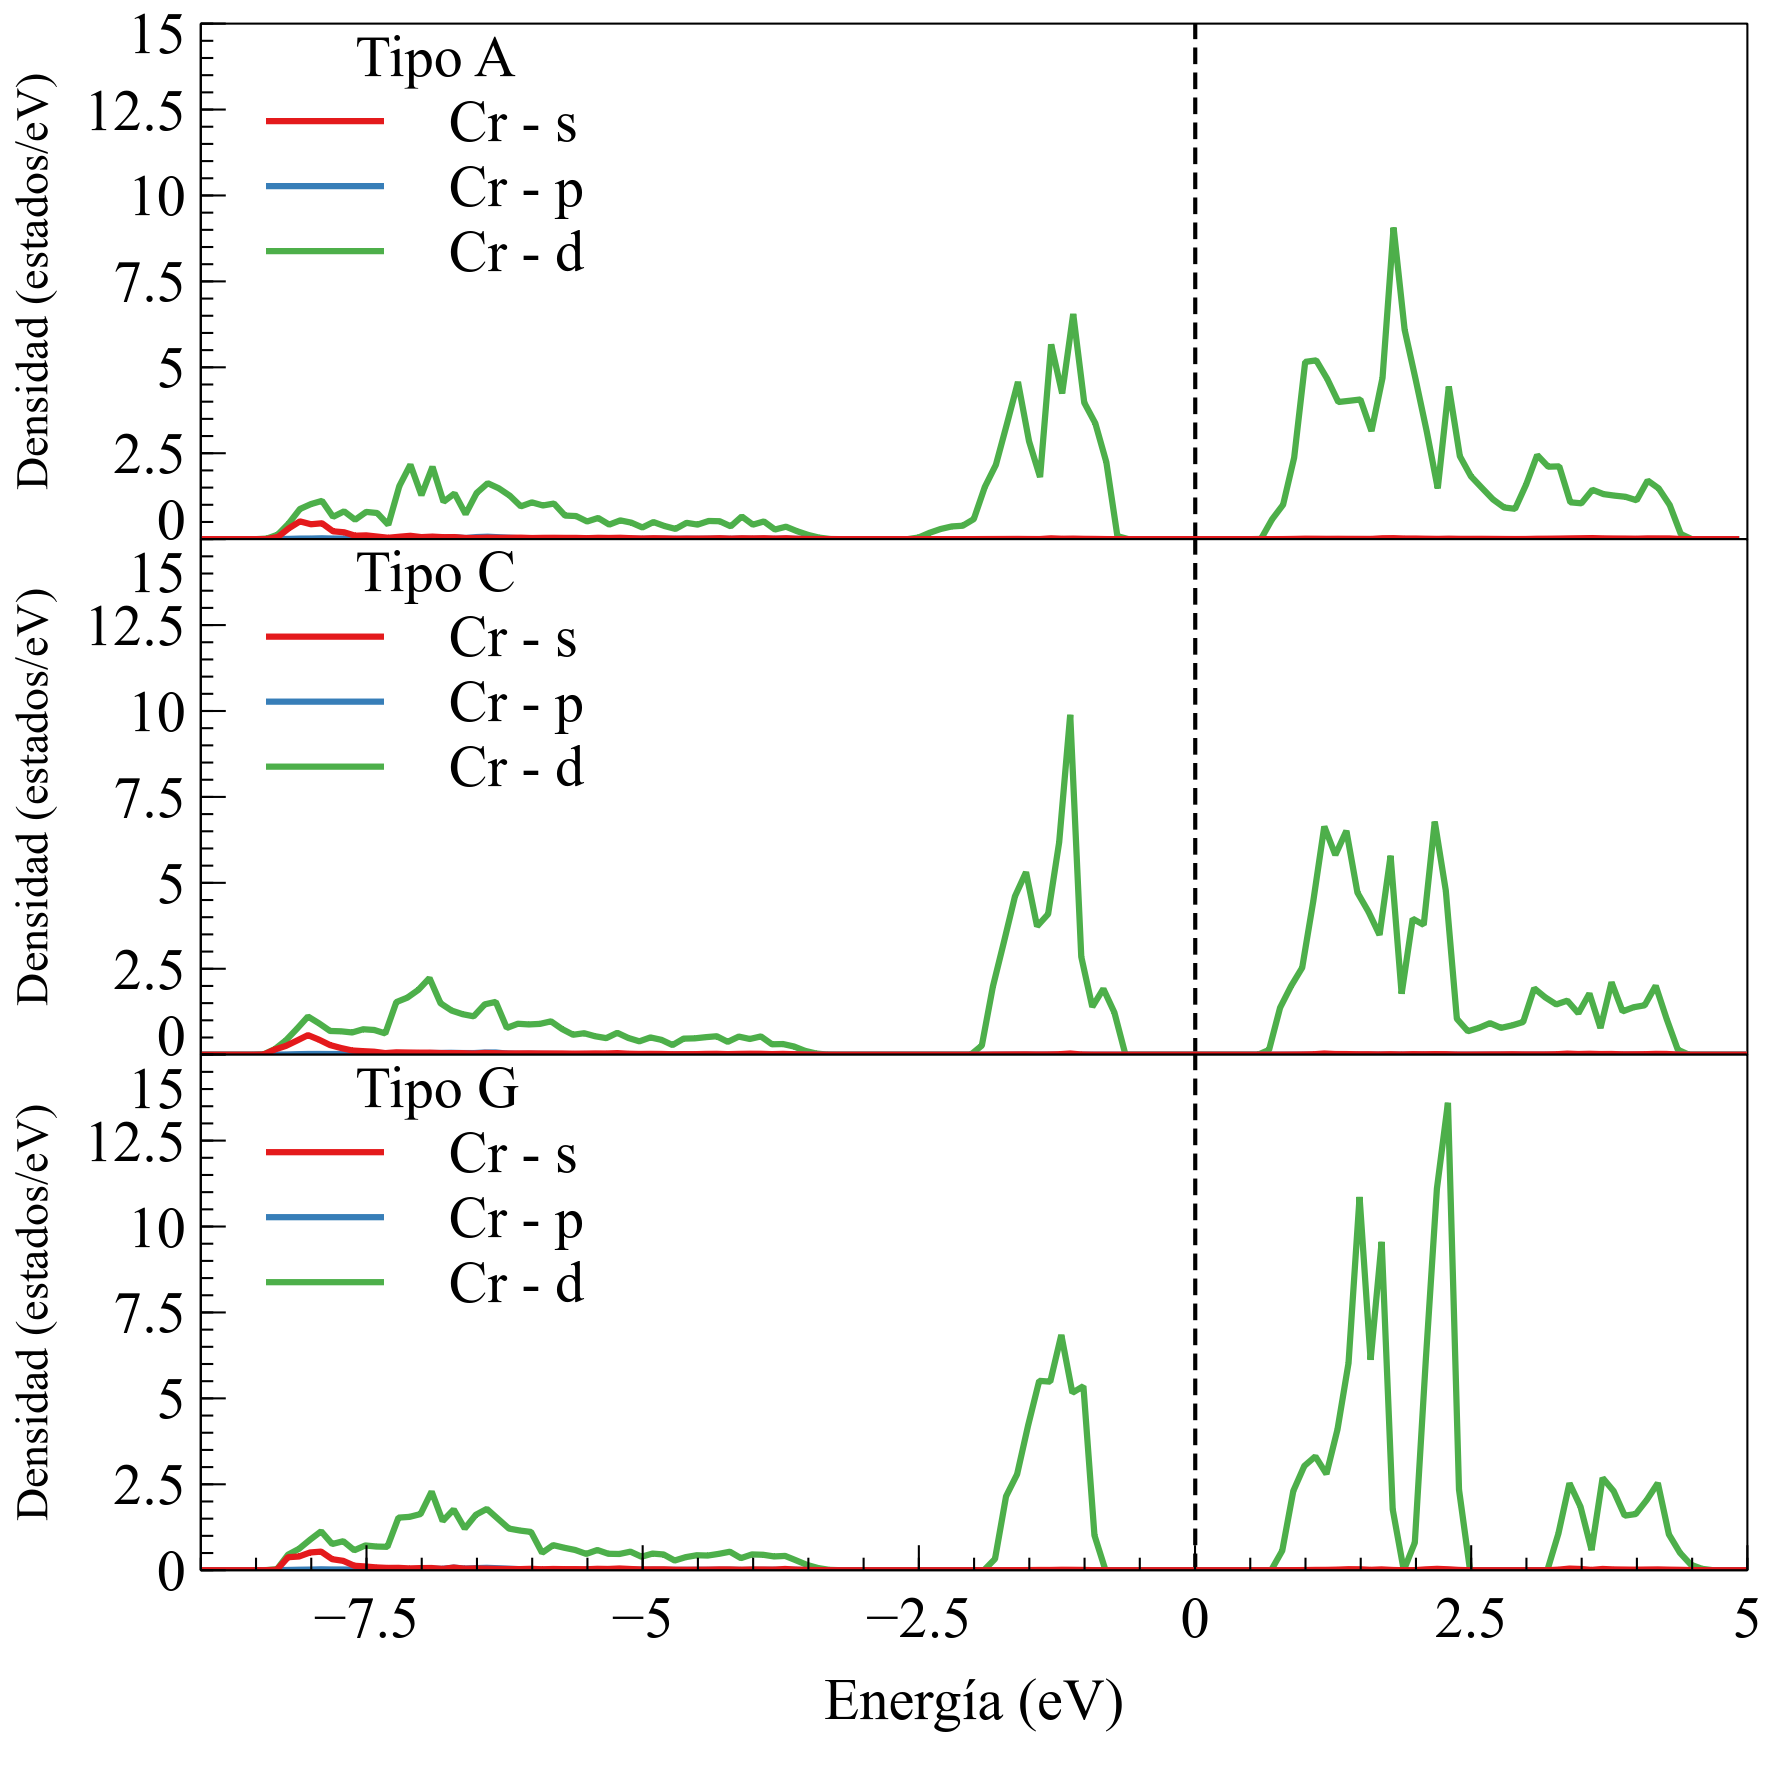
\includegraphics[width=1.0\textwidth]{contenido/resultados/img_resultados/YCO_Cr_tipos.png}
        \caption{Densidad de estados parcial del cromo del $YCrO_{3}$.}
    \end{figure}
\end{columns}
\end{frame}

\begin{frame}
     \begin{figure}[H]
    \centering
    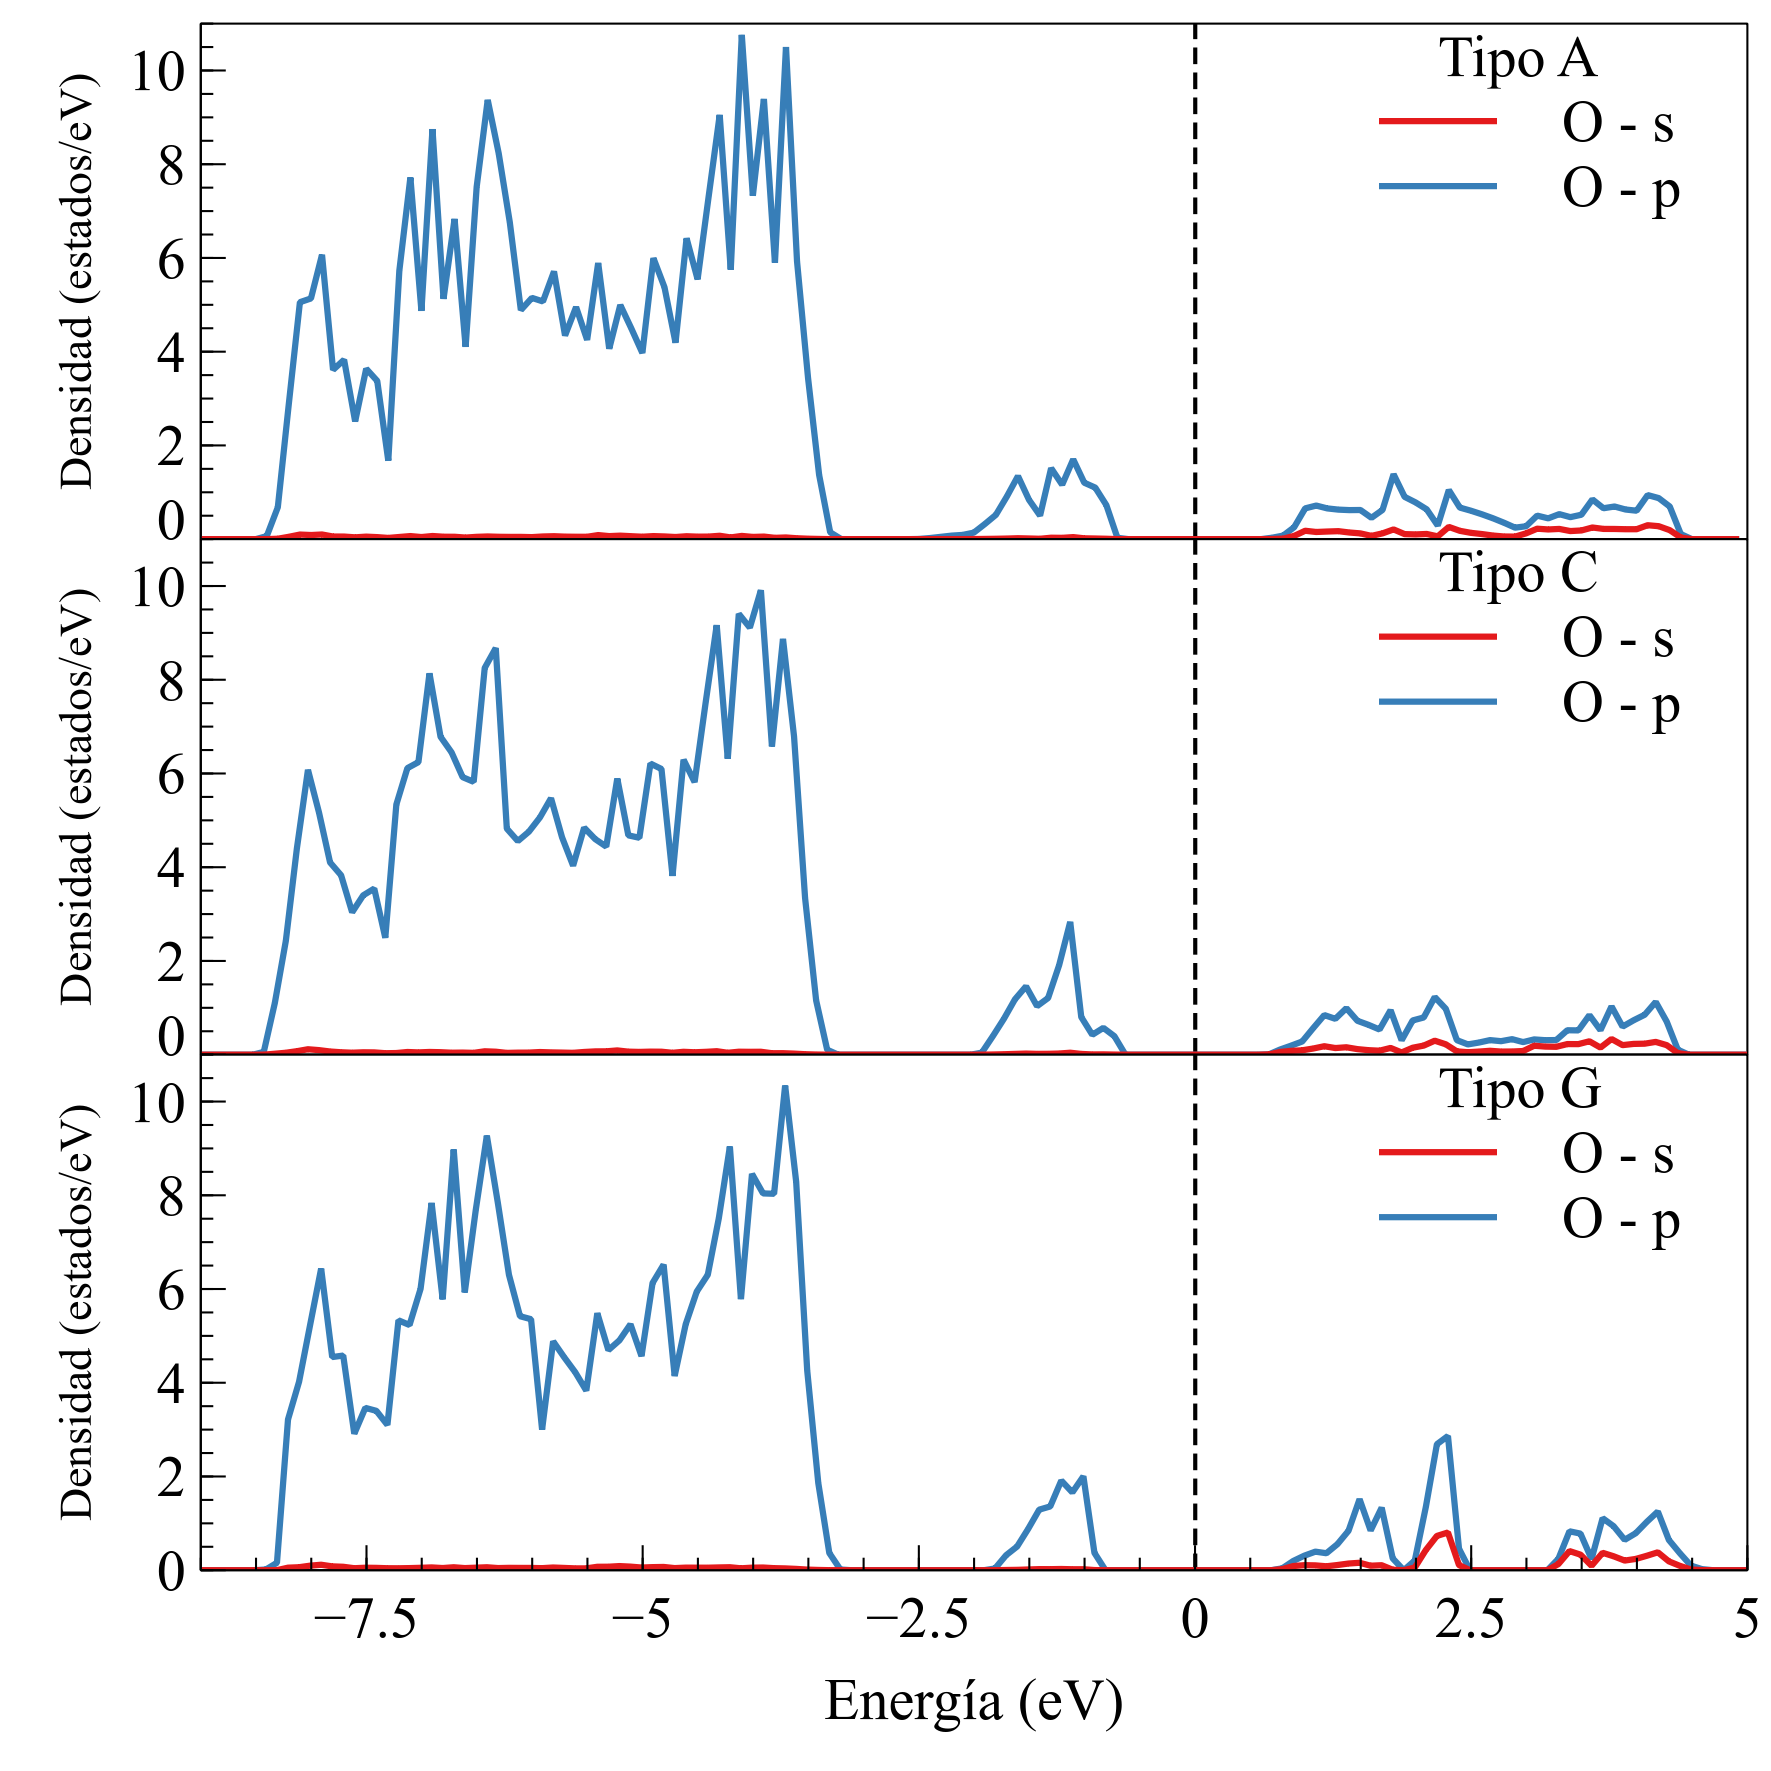
\includegraphics[width=0.5\textwidth]{contenido/resultados/img_resultados/YCO_O_tipos.png}
    \caption{Densidad de estados parcial del ox\'igeno del $YCrO_{3}$.}
    \end{figure}
\end{frame}

\subsection{Comparaci\'on}
\begin{frame}{Comparaci\'on entre $BiFeO_{3}$ y $YCrO_{3}$}
    \begin{table}[H]
        \begin{center}
            \caption{Comparaci\'on entre los gap de energ\'ia del $BiFeO_{3}$ y del $YCrO_{3}$.}
            \begin{tabular}{ccp{2cm}cp{2cm}}
                \hline
                & $BiFeO_{3}$&  & $YCrO_{3}$ &  \\
                \hline \hline
                Tipo A & $1.4$&  & $1.3$ &   \\
                \hline
                Tipo G & $1.8$& $1.9$ S. Ju et al. Chem. Phys. 130, 2009 & $1.6$ & $1.8$ Serrao et al. Physical Review B, 72, 2005 \\
                \hline
                Tipo C &  &  & $1.32$ &  \\
                \hline
            \end{tabular}
        \end{center}
    \end{table}
\end{frame}

% #####            #####
%       CONCLUSION
% #####            ##### 
\section{Conclusiones}

\begin{frame}{Conclusiones}
    \begin{itemize}
    	\item Se han realizado con \'exito c\'alculos de estructura electr\'onica para el $BiFeO_{3}$ y el $YCrO_{3}$.
        \item Para el $BiFeO_{3}$ se observaron gaps de energ\'ia de $1.4$ eV y 
        $1.8$ eV para los arreglos antiferromagn\'eticos tipo A y G 
        respectivamente.
         \item Los orbitales \textbf{d} del hierro poseen la mayor densidad 
         cerca del nivel de fermi en la banda de conducci\'on.
        \item Para el $YCrO_{3}$ se observaron gaps de energ\'ia de $1.3$ eV, 
        $1.32$ eV y $1.6$ eV para los arreglos antiferromagn\'eticos tipo A, C 
        y G respectivamente.
        \item Los orbitales \textbf{d} del cromo poseen la mayor densidad cerca 
        del nivel de fermi en la banda de conducci\'on y en la banda de 
        valencia.
    \end{itemize}
\end{frame}

\begin{frame}
    Esta tesis a dado lugar a los siguientes trabajos:
    \begin{itemize}
        \item Un poster en XVII Encuentro de F\'isica.
        \item Un poster en XXVII Simposio Peruano de F\'isica.
        \item Un art\'iculo en la revista REVCIUNI.
    \end{itemize}
\end{frame}

\begin{frame}
    
\end{frame}

\end{document}